\documentclass[aspectratio=169]{beamer}

\usetheme{metropolis}

\usepackage{amsmath}
\usepackage{amssymb}
\usepackage{amsthm}
\usepackage{mathtools}
\usepackage{xcolor}
\usepackage{physics}
\usepackage{bm}
\usepackage{tikz}
\usepackage{pgfplots}
\pgfplotsset{compat=1.18}
\usepackage{svg}
\usepackage{graphicx}
\usepackage{subcaption}
\usepackage{minted}
\usepackage{nicematrix}
\usepackage{verbatim}

\usetikzlibrary{arrows.meta, positioning}
\usemintedstyle{monokai}
\newcommand{\dimterm}[2]{\alt<1>{#2}{\alt<#1>{#2}{{\color{black!20}#2}}}}

\title{Simulating lid-driven cavity}
\author{Lukas Lanik}
\date{\today}

\begin{document}

\begin{frame}
  \titlepage
\end{frame}

\begin{comment}
\begin{frame}{\Large The problem at hand}
  \begin{figure}[htbp]
    \centering
    \begin{subfigure}[b]{0.45\textwidth}
      \centering
      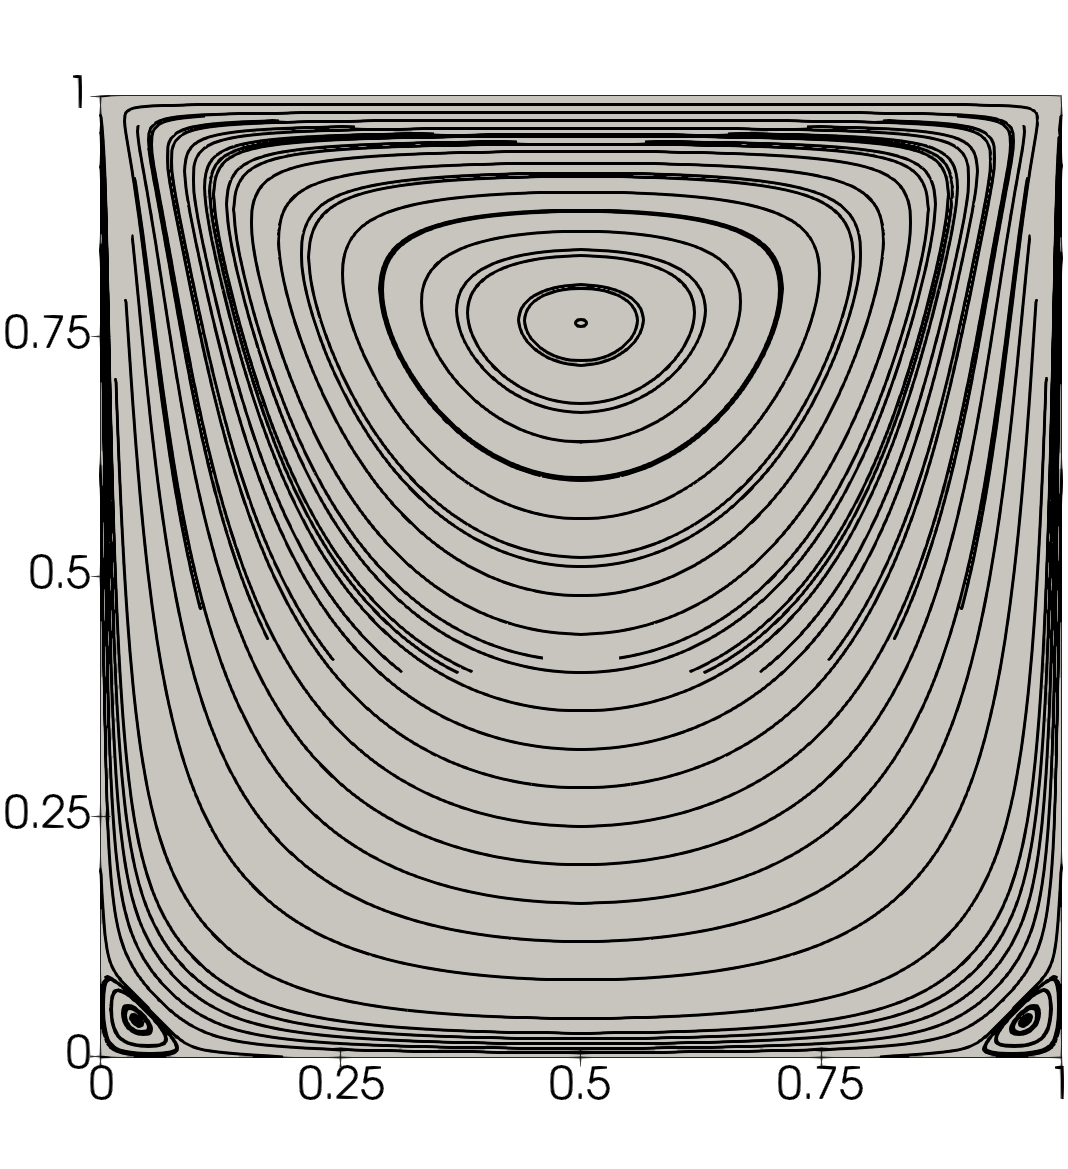
\includegraphics[width=\textwidth]{./images/cavity_P2-P1_128_velocity.png}
      \caption{Velocity streamlines}
      \label{problem:first_image}
    \end{subfigure}
    \begin{subfigure}[b]{0.45\textwidth}
      \centering
      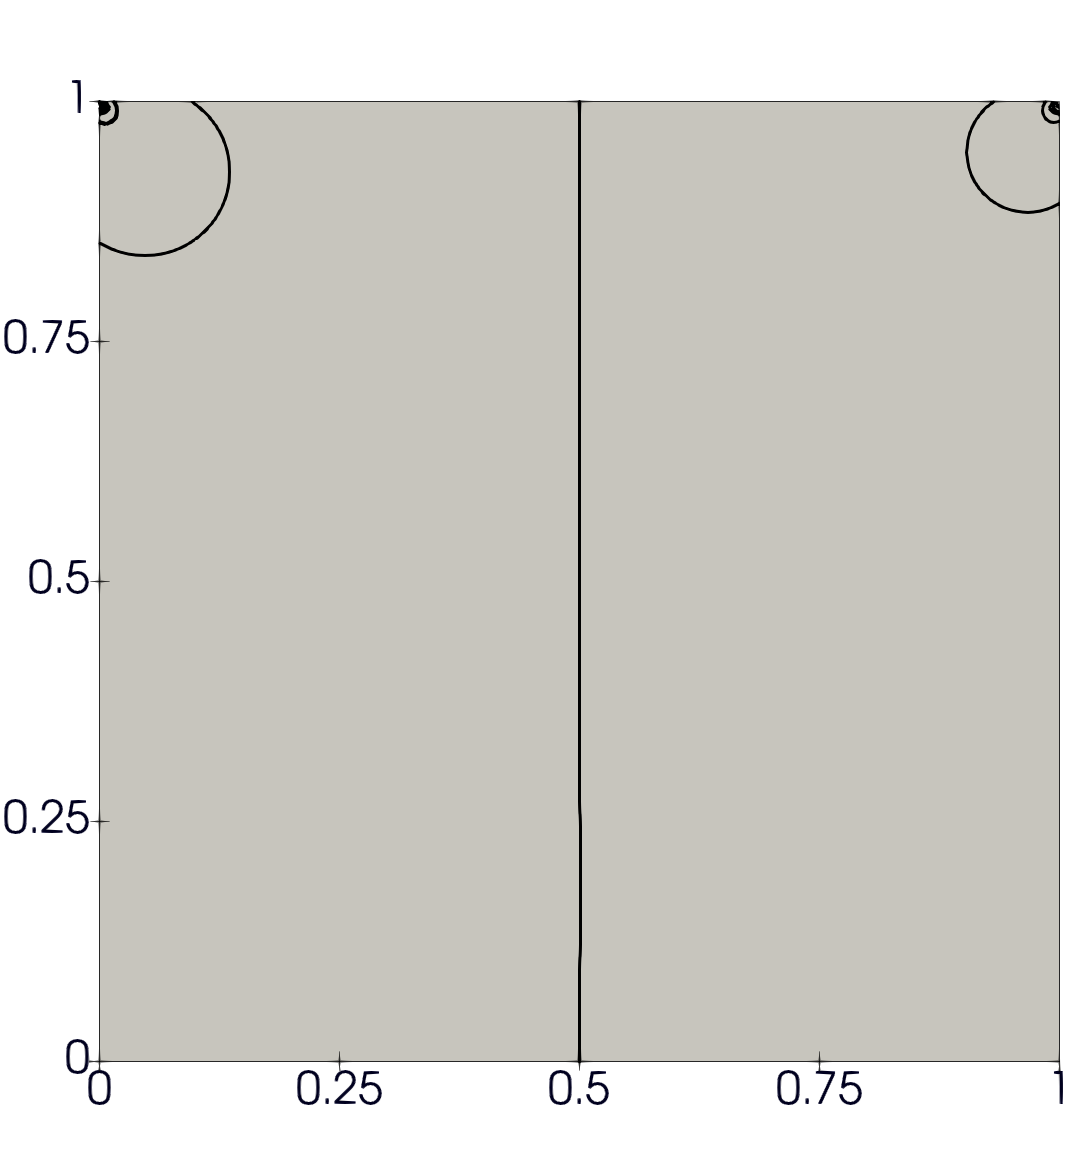
\includegraphics[width=\textwidth]{./images/cavity_P2-P1_128_pressure.png}
      \caption{Pressure isolines}
      \label{problem:second_image}
    \end{subfigure}
  \end{figure}
\end{frame}
\end{comment}

\begin{frame}{\Large The problem at hand}
  \Large
  Simulating the flow of a viscuous fluid in a 2D cavity
\begin{center}
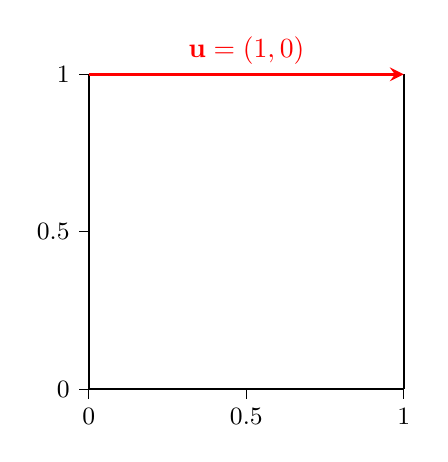
\begin{tikzpicture}[scale=4]
    % Draw grid / ticks
    \draw[help lines, color=gray!30, dashed] (0,0) grid (1,1);
    
    % Axis ticks along the bottom and left edges
    \foreach \x in {0, 0.5, 1}
        \draw (\x,0) -- (\x,-0.03) node[below] {\small\x};
    \foreach \y in {0, 0.5, 1}
        \draw (0,\y) -- (-0.03,\y) node[left] {\small\y};

    % Square outline (bottom, left, and right edges)
    \draw[thick] (0,0) -- (1,0); % bottom
    \draw[thick] (0,0) -- (0,1); % left
    \draw[thick] (1,0) -- (1,1); % right

    % Top edge as a red arrow pointing to the right
    \draw[red, very thick, -stealth] (0,1) -- (1,1);

    % Label the red arrow with u = (1, 0)
    \node[above, red] at (0.5, 1) {$\mathbf{u} = (1, 0)$};
\end{tikzpicture}
\end{center}
\end{frame}

\begin{frame}{\Large Stokes problem}
  \Large
  \begin{equation*}
    \begin{cases}
      -\Delta \mathbf{u} 
      + \nabla p = 0, & \mathbf{x} \in \Omega \\[5pt]
      \operatorname{div} \mathbf{u} = 0, & \mathbf{x} \in \Omega
    \end{cases}
  \end{equation*}
  \begin{align*}
    \mathbf{u} &= \mathbf{0}, \qquad\mathbf{x} \in \partial\Omega \setminus \varGamma, \\[5pt]
    \mathbf{u} &= (1,0)^T, \qquad \mathbf{x} \in \varGamma,
  \end{align*}
  \centering
  where $\varGamma = \{\mathbf{x} = (x_1, x_2)^T \in \partial \Omega: x_2 = 1\}$
\end{frame}

\begin{frame}{\Large Solution methods}
  \Large
  \begin{itemize}
    \item Finite difference/ Staggered MAC
    \item Spectral methods
    \item Finite Element Method
  \end{itemize}
\end{frame}

\begin{frame}{\Large Solution methods}
  \Large
  All of the methods create a system
  \begin{equation*}
  \begin{pmatrix}
    A & B^{T} \\
    B & 0
  \end{pmatrix}
  \begin{pmatrix}
    \mathbf{U} \\
    \mathbf{P}
  \end{pmatrix}
  =
  \begin{pmatrix}
    \mathbf{f} \\
    \mathbf{g}
  \end{pmatrix}
  \end{equation*}
\end{frame}

\begin{frame}{\Large Finite difference/ Staggered MAC}
\centering
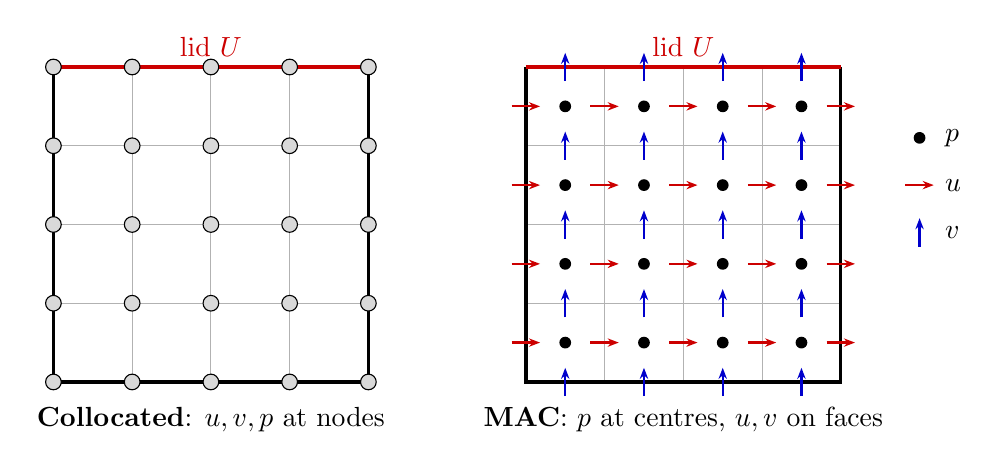
\begin{tikzpicture}[
  pnode/.style  = {circle, fill=black, inner sep=1.5pt},
  cnode/.style  = {circle, draw, fill=gray!30, inner sep=2pt},
  uarr/.style   = {red!80!black, thick, -{Stealth[length=4pt]}},
  varr/.style   = {blue!80!black, thick, -{Stealth[length=4pt]}}]

  % ---------- Collocated grid ----------
  \draw[gray!60] (0,0) grid (4,4);
  \draw[very thick] (0,4) -- (0,0) -- (4,0) -- (4,4);
  \draw[very thick, red!80!black] (0,4) -- (4,4) node[midway, above] {lid $U$};
  \foreach \i in {0,...,4} \foreach \j in {0,...,4}
    \node[cnode] at (\i,\j) {};
  \node[below] at (2,-0.2) {\textbf{Collocated}: $u,v,p$ at nodes};

  % ---------- MAC grid ----------
  \begin{scope}[xshift=6cm]
    \draw[gray!60] (0,0) grid (4,4);
    \draw[very thick] (0,4) -- (0,0) -- (4,0) -- (4,4);
    \draw[very thick, red!80!black] (0,4) -- (4,4) node[midway, above] {lid $U$};
    \foreach \i in {1,...,4} \foreach \j in {1,...,4}
      \node[pnode] at (\i-0.5,\j-0.5) {};                          % p
    \foreach \i in {0,...,4} \foreach \j in {1,...,4}
      \draw[uarr] (\i-0.18,\j-0.5) -- (\i+0.18,\j-0.5);           % u
    \foreach \i in {1,...,4} \foreach \j in {0,...,4}
      \draw[varr] (\i-0.5,\j-0.18) -- (\i-0.5,\j+0.18);           % v
    \node[below] at (2,-0.2) {\textbf{MAC}: $p$ at centres, $u,v$ on faces};
  \end{scope}

  % ---------- Legend ----------
  \begin{scope}[xshift=11cm, yshift=2.5cm]
    \node[pnode] at (0,0.6) {};            \node[right] at (0.2,0.6)  {$p$};
    \draw[uarr] (-0.18,0) -- (0.18,0);     \node[right] at (0.2,0)    {$u$};
    \draw[varr] (0,-0.78) -- (0,-0.42);    \node[right] at (0.2,-0.6) {$v$};
  \end{scope}
\end{tikzpicture}
\end{frame}

\begin{frame}{\Large Finite difference}
  \Large
  \[
\begin{aligned}
  -(\Delta_h u_1)_{i,j} + \frac{p_{i+1,j}-p_{i-1,j}}{2h} &= 0, \\
  -(\Delta_h u_2)_{i,j} + \frac{p_{i,j+1}-p_{i,j-1}}{2h} &= 0, \\
  \frac{(u_1)_{i+1,j}-(u_1)_{i-1,j}}{2h} + \frac{(u_2)_{i,j+1}-(u_2)_{i,j-1}}{2h} &= 0,
\end{aligned}
\]
\begin{center}
  with $\mathbf{u}_{i,j} = (1,0)^T$ on $\Gamma$ and $\mathbf{u}_{i,j} = \mathbf{0}$ on $\partial\Omega\setminus\Gamma$.
\end{center}
\end{frame}

\begin{frame}{\Large Staggered MAC}
  \Large
\[
\begin{aligned}
  -(\Delta_h u_1)_{i+\frac12,j} + \frac{p_{i+1,j}-p_{i,j}}{h} &= 0, \\
  -(\Delta_h u_2)_{i,j+\frac12} + \frac{p_{i,j+1}-p_{i,j}}{h} &= 0, \\
  \frac{(u_1)_{i+\frac12,j}-(u_1)_{i-\frac12,j}}{h} + \frac{(u_2)_{i,j+\frac12}-(u_2)_{i,j-\frac12}}{h} &= 0,
\end{aligned}
\]
\begin{center}
  with ghost values $(u_1)_{\text{ghost}} = 2 - (u_1)_{\text{interior}}$ on $\Gamma$.
\end{center}
\end{frame}

\begin{frame}{\Large Spectral Methods}
  \centering
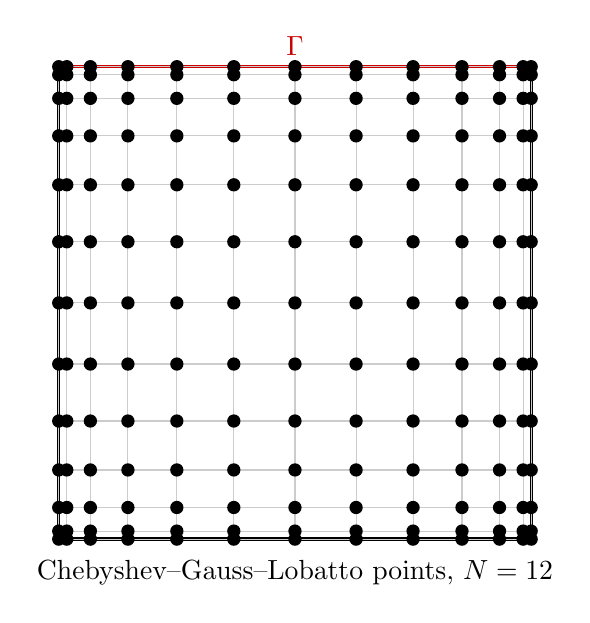
\begin{tikzpicture}[scale=3]
  \def\N{12}
  \draw[very thick] (-1,1) -- (-1,-1) -- (1,-1) -- (1,1);
  \draw[very thick, red!80!black] (-1,1) -- (1,1) node[midway, above] {$\Gamma$};
  \foreach \i in {0,...,\N} {
    \draw[gray!40] ({cos(180*\i/\N)},-1) -- ({cos(180*\i/\N)},1);
    \draw[gray!40] (-1,{cos(180*\i/\N)}) -- (1,{cos(180*\i/\N)});
  }
  \foreach \i in {0,...,\N} \foreach \j in {0,...,\N}
    \fill ({cos(180*\i/\N)},{cos(180*\j/\N)}) circle (0.8pt);
  \node[below] at (0,-1.05) {Chebyshev--Gauss--Lobatto points, $N=12$};
\end{tikzpicture}
\end{frame}

\begin{frame}{\Large Spectral Methods}
  \Large
\[
  u_{1}^N(\mathbf{x}) = \sum_{k,l=0}^{N} \hat u_{kl}\,T_k(x_1)\,T_l(x_2),
  \qquad
  p^N(\mathbf{x}) = \sum_{k,l=0}^{N-2} \hat p_{kl}\,T_k(x_1)\,T_l(x_2),
\]
\begin{center}
  similarly for $u_2^N$, with $T_k(\cos\theta) = \cos(k\theta)$.
\end{center}
\end{frame}

\begin{frame}{\Large Finite Element Method}
  \Large
  Let $\mathbf{v} \in V$ and $q \in Q$, find $\mathbf{u} \in V$, $p \in Q$ such that
  \begin{equation*}
    V = \{ \mathbf{v} \in \left[ \mathrm{H}^1 (\Omega) \right]^2 : \mathbf{v} \vert_{\varGamma_D} = 0 \}
  \end{equation*}
  \begin{equation*}
    Q = \{q \in \mathrm{L}^2 (\Omega) : \int_{\Omega} q \, d\Omega = 0 \}
  \end{equation*}
  \begin{equation*}
    \int_{\Omega} \nabla \mathbf{u} \cdot \nabla \mathbf{v} \, d\Omega 
    -\int_{\Omega} p \operatorname{div} \mathbf{v} \, d\Omega 
    = 0
  \end{equation*}
  \begin{equation*}
    \int_{\Omega} (\operatorname{div} \mathbf{u}) \, q \, d\Omega = 0
  \end{equation*}
\end{frame}

\begin{frame}{\Large Galerkin approximation}
  \Large
  Let $V_h \subset V$, $Q_h \subset Q$ be finite dimensional subspaces. Find
  $u_h = \sum_{i=0}^{N_h} u_i \varphi_i$,
  $p_h = \sum_{k=0}^{M_h} p_k \phi_k$.

  The Stokes problem becomes
  \begin{equation*}
    \begin{cases}
      \mathsf{A}\mathbf{U} + \mathsf{B}^T \mathbf{P} = 0 \\
      \mathsf{B} \mathbf{U} = 0
    \end{cases}
  \end{equation*}
  
  \begin{equation*}
    \mathsf{A} = [a_{ij}] = [a(\varphi_j, \varphi_i)], \quad \mathsf{B} = [b_{km}] = [b(\varphi_m, \phi_k)] 
  \end{equation*}
\end{frame}

\begin{comment}
\begin{frame}{\Large Why choose FEM?}
  \Large
  \begin{itemize}
    \item other methods: Finite Volume, Finite Difference, Spectral Methods
    \item general geometry vs strict geometry (rectangle, polyhedra)
    \item mature FEM infrastructure in place
    \item build upon acquired knowledge in previous course
  \end{itemize}
\end{frame}
\end{comment}

\begin{frame}{\Large Meshing}
\begin{columns}[c] % [c] vertically centers the content in both columns
    
    % --- Left Column: Image ---
    \begin{column}{0.48\textwidth}
      \centering
      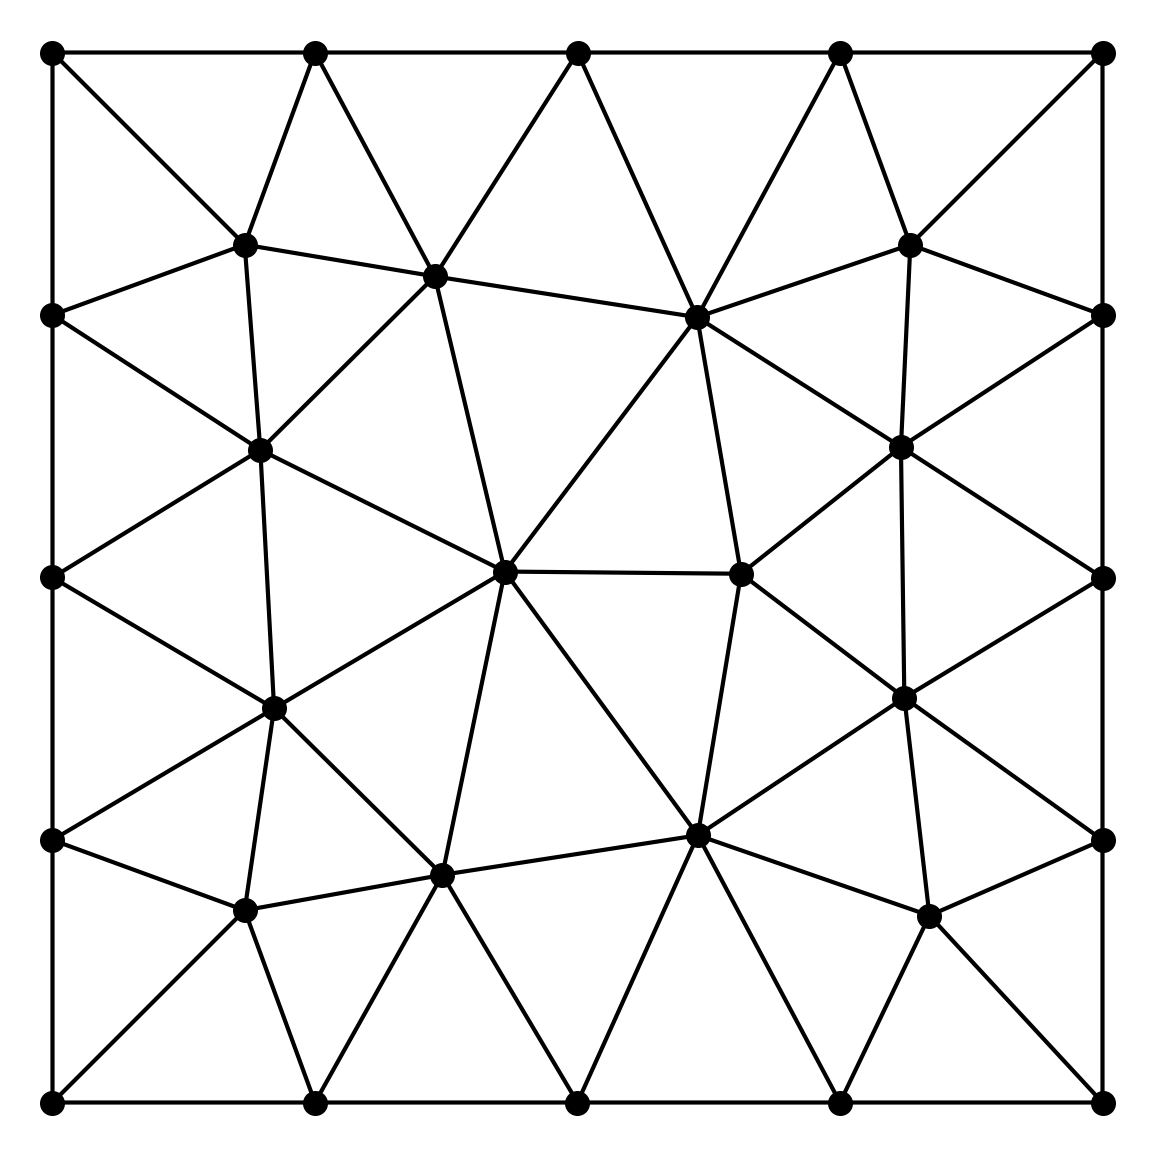
\includegraphics[width=\textwidth]{./images/example_mesh.png} % Replace with your image file
    \end{column}

    % --- Right Column: Bullet Points ---
    \begin{column}{0.48\textwidth}
      \Large
      \begin{itemize}
        \item choose target mesh size $h$ (size of an edge)
        \item non-overlapping
        \item unstructured
      \end{itemize}
    \end{column}

  \end{columns}
\end{frame}

\iffalse
\begin{frame}{\Large Structured/Unstructured meshes}
    \begin{figure}[htbp]
    \centering
    \begin{subfigure}[b]{0.45\textwidth}
      \centering
      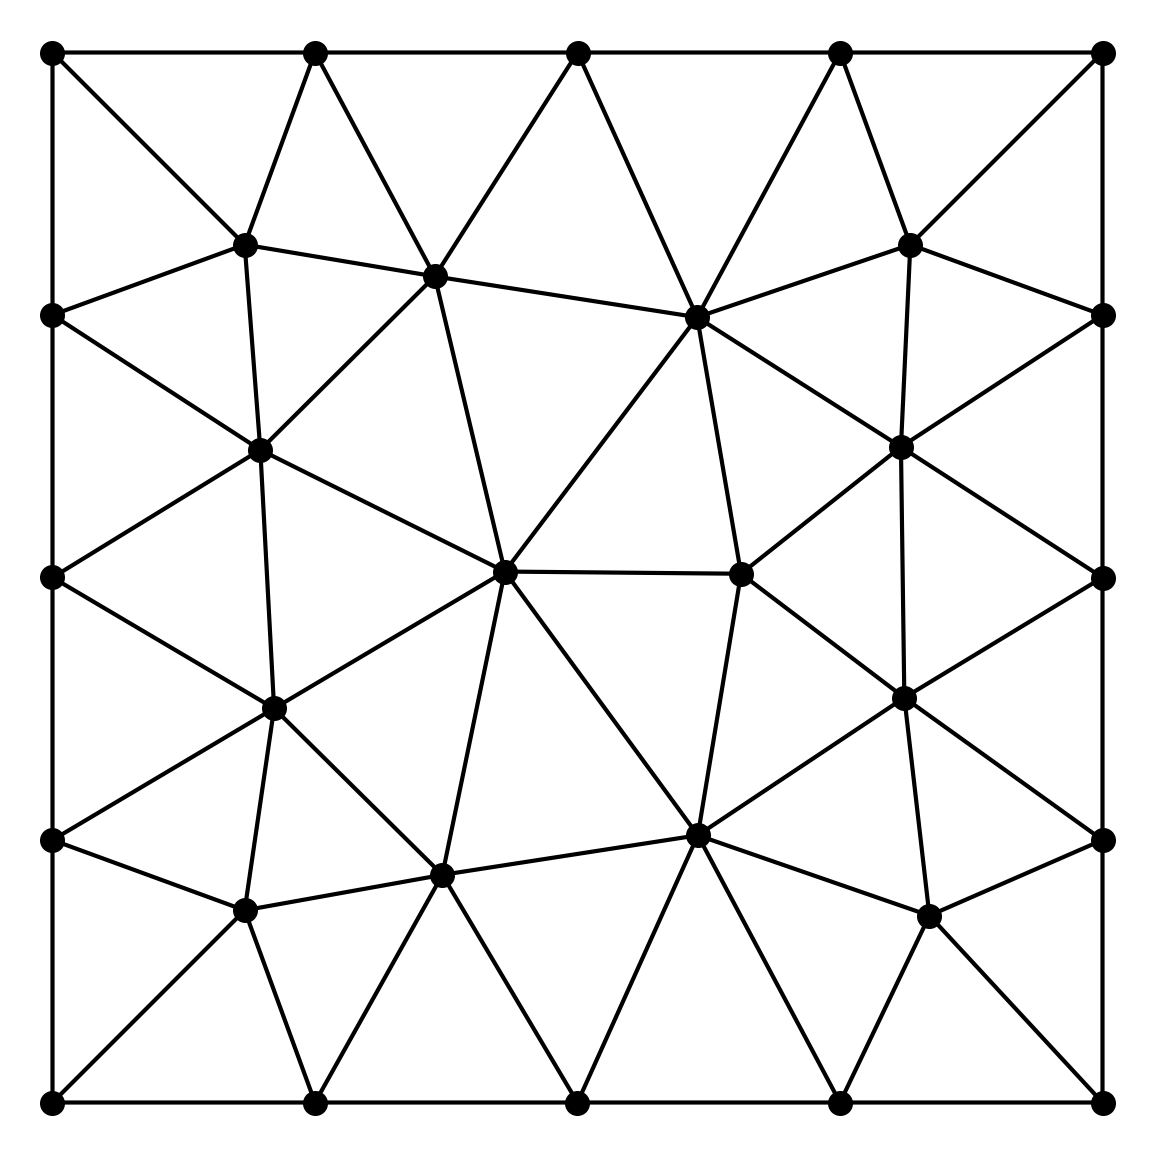
\includegraphics[width=\textwidth]{./images/example_mesh.png}
      \caption{Unstructured mesh}
      \label{mesh_structure:first_image}
    \end{subfigure}
    \begin{subfigure}[b]{0.45\textwidth}
      \centering
      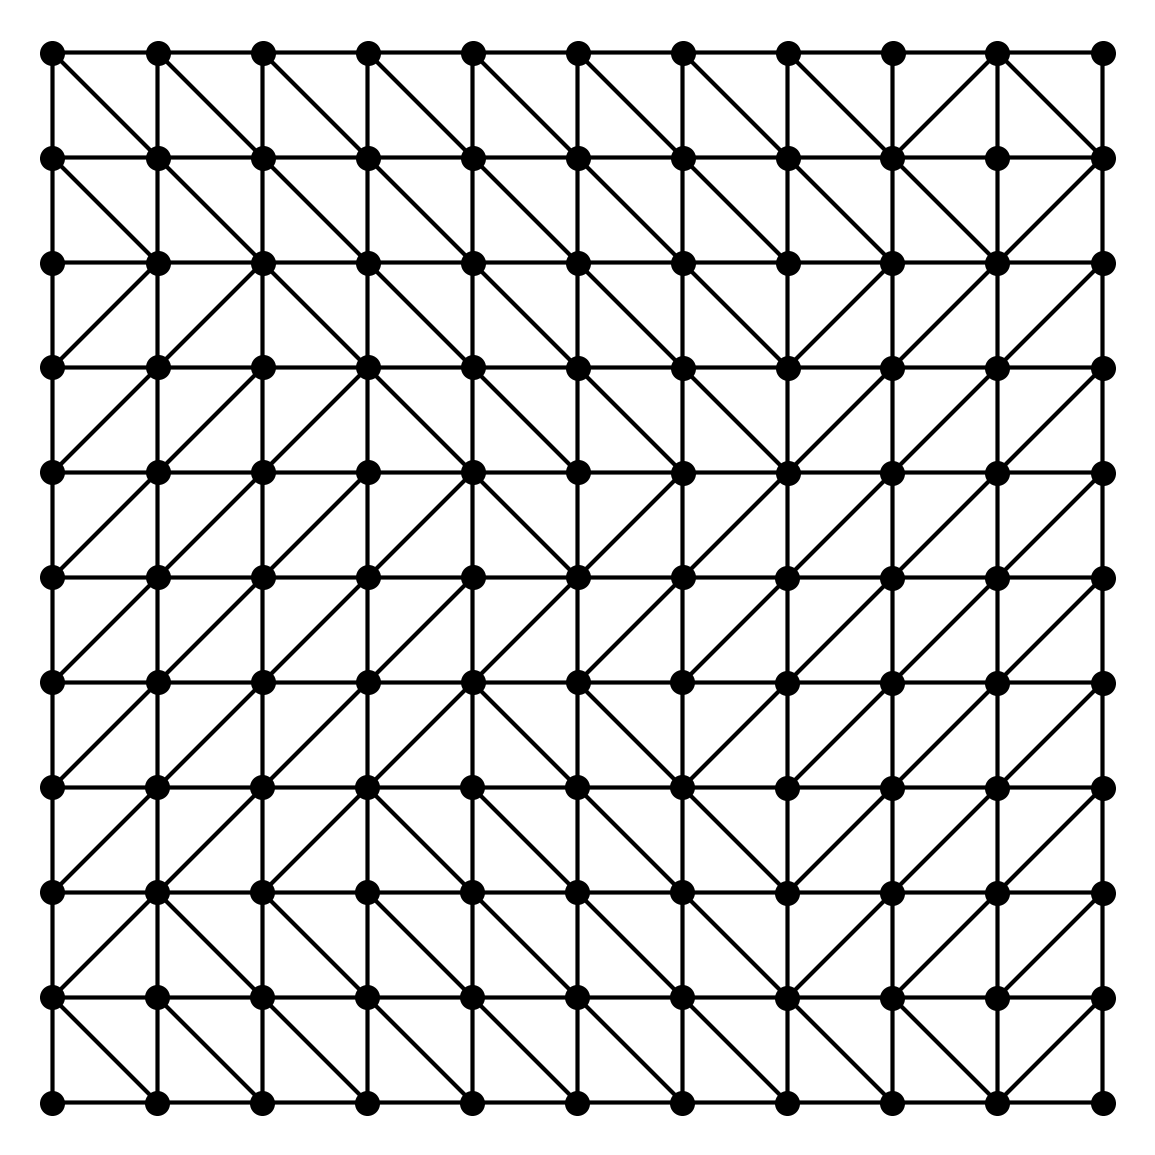
\includegraphics[width=\textwidth]{./images/structured_mesh.png}
      \caption{Structured mesh}
      \label{mesh_structure:second_image}
    \end{subfigure}
  \end{figure}
\end{frame}
\fi

\begin{comment}
\begin{frame}{\Large Meshing algorithms}
  \begin{figure}[htbp]
    \centering
    \begin{subfigure}[b]{0.45\textwidth}
      \centering
      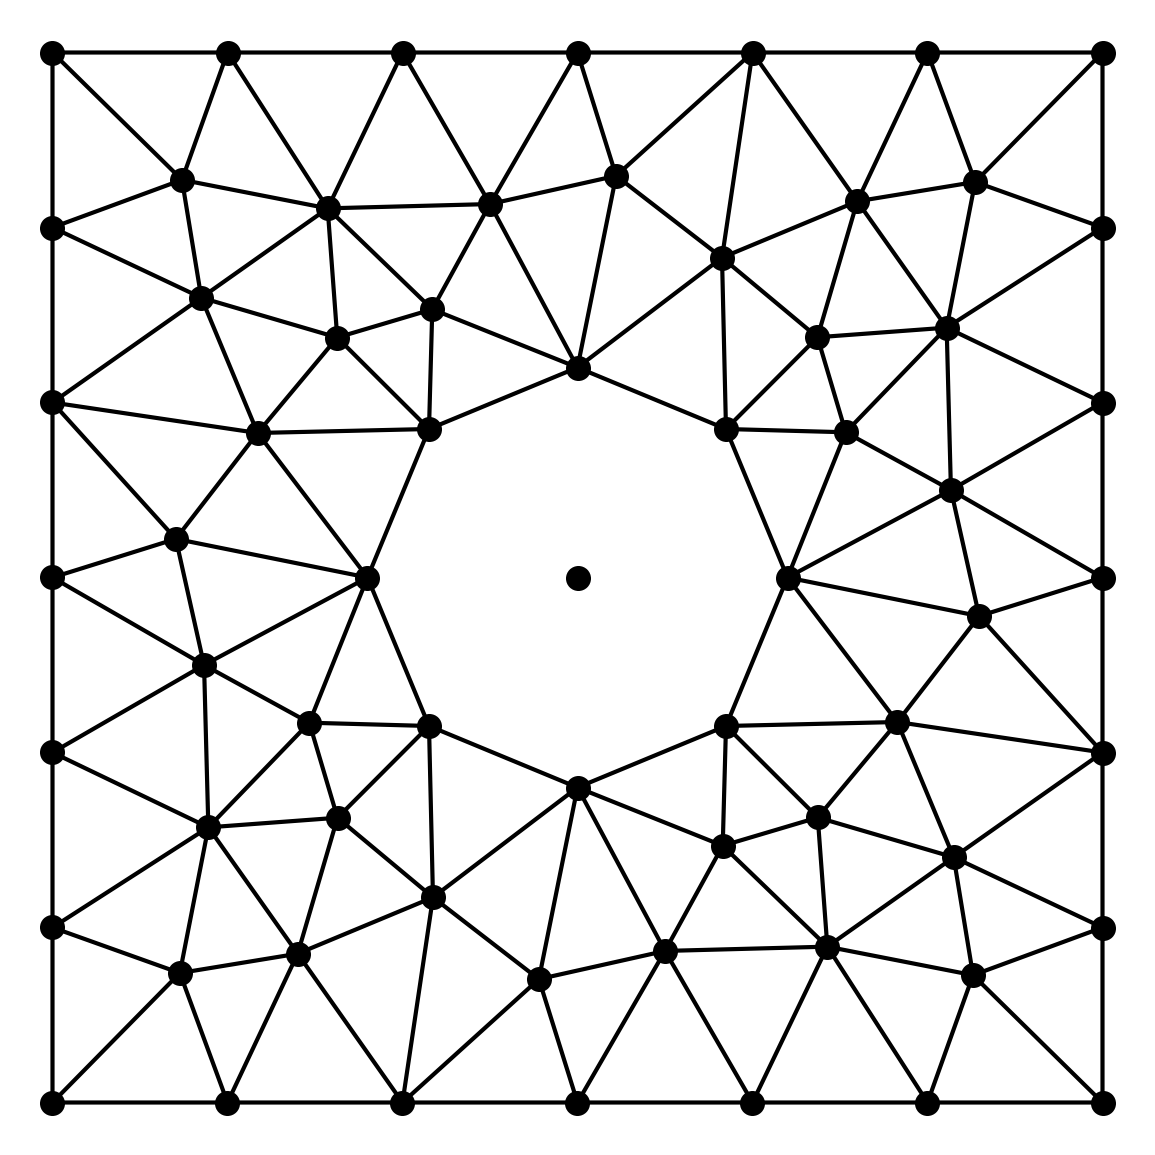
\includegraphics[width=\textwidth]{./images/delunay_mesh.png}
      \caption{Delunay algorithm}
      \label{mesh_algo:first_image}
    \end{subfigure}
    \begin{subfigure}[b]{0.45\textwidth}
      \centering
      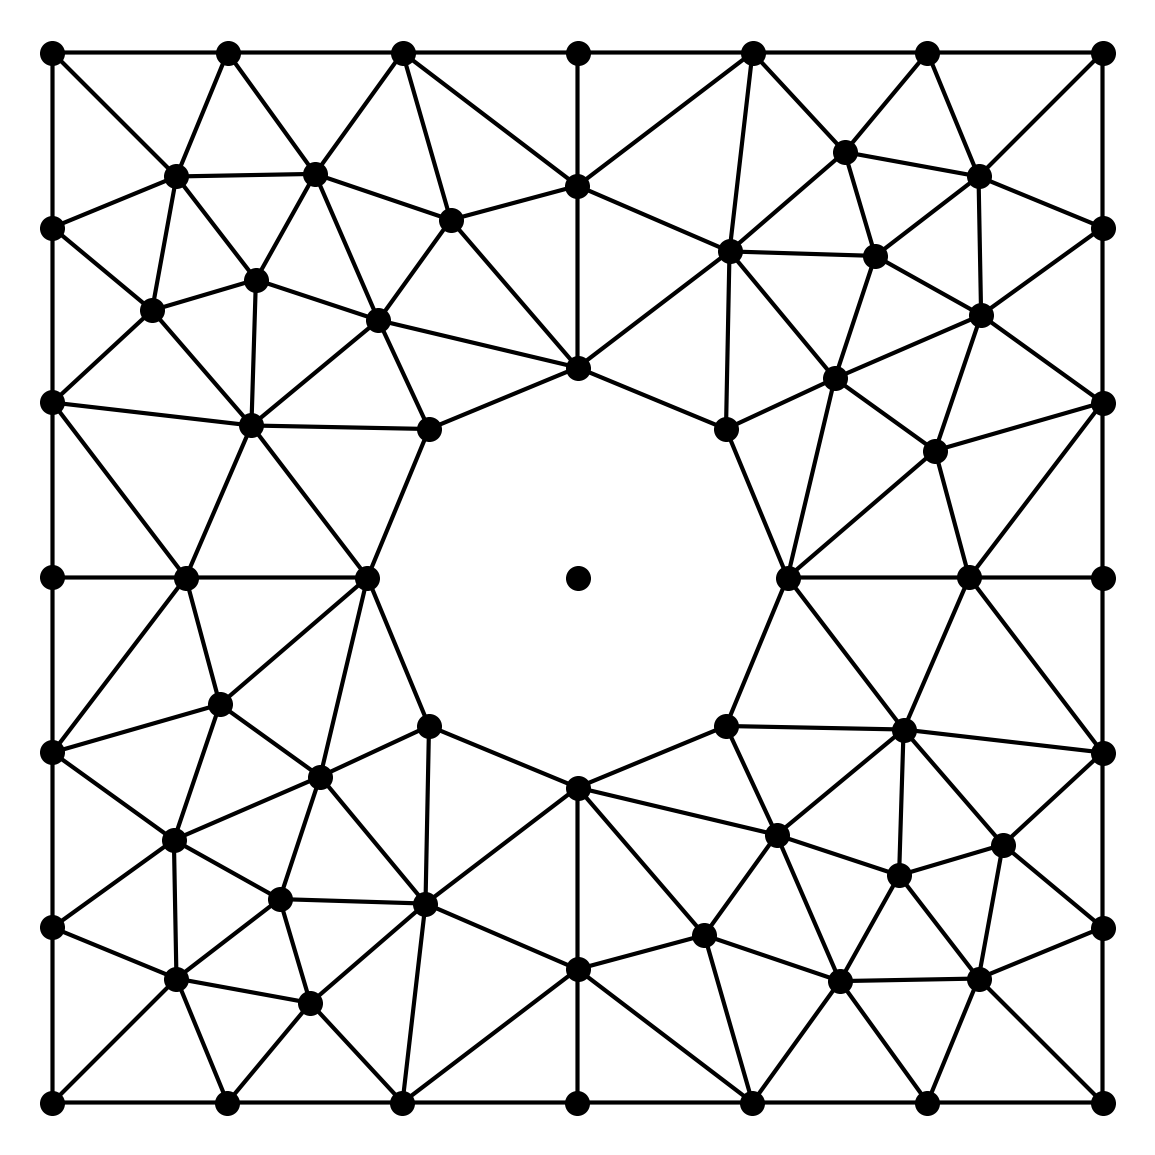
\includegraphics[width=\textwidth]{./images/advancing_front.png}
      \caption{Advancing front}
      \label{mesh_algo:second_image}
    \end{subfigure}
  \end{figure}
\end{frame}
\end{comment}

\begin{frame}{\Large FEniCSx}
  \Large
  \begin{itemize}
    \item computation of PDEs
    \item DOLFINX, UFL, FFCx, Basix
    \item variational form $\rightarrow$ matrix
    \item C++ with python bindings
  \end{itemize}
\end{frame}

\begin{frame}[fragile]{\Large Code setup}
\begin{minted}[
    backgroundcolor=black!85,
    frame=lines,      % Frame lines top and bottom
    framesep=2mm
  ]{python}
  from dolfinx import fem

  V = fem.functionspace(mesh, ("Lagrange", 2, (2,)))
  Q = fem.functionspace(mesh, ("Lagrange", 1))

  u = ufl.TrialFunction(V)
  v = ufl.TestFunction(V)
  p = ufl.TrialFunction(Q)
  q = ufl.TestFunction(Q)
  \end{minted}
\end{frame}

\begin{frame}[fragile]{\Large Code setup}
\begin{minted}[
    backgroundcolor=black!85,
    frame=lines,      % Frame lines top and bottom
    framesep=2mm
  ]{python}
  a00 = ufl.inner(ufl.grad(u), ufl.grad(v)) * ufl.dx
  a01 = -p * ufl.div(v) * ufl.dx
  a10 = -q * ufl.div(u) * ufl.dx
  a11 = None

  L0 = ufl.inner(f0, v) * ufl.dx
  L1 = f1 * q * ufl.dx
  \end{minted}
\end{frame}


\begin{frame}{\Large Boundary conditions}
  \Large
  Assemble the full system first:
  \begin{equation*}
  \begin{bmatrix} A_{ff} & A_{fb} \\ A_{bf} & A_{bb} 
    \end{bmatrix} 
    \begin{bmatrix} u_f \\ u_b \end{bmatrix} 
      = \begin{bmatrix} b_f \\ b_b 
      \end{bmatrix}
  \end{equation*}
  
  afterwards apply boundary conditions:
  \begin{equation*}
    \Rightarrow
    \begin{bmatrix} 
      A_{ff} & 0 \\ 0 & I 
    \end{bmatrix} 
    \begin{bmatrix} 
      u_f \\ u_b 
      \end{bmatrix} 
      = \begin{bmatrix} 
      b_f - A_{fb} u_D \\ u_D 
    \end{bmatrix}
  \end{equation*}
\end{frame}

\begin{frame}{\Large Matrix assembly}
  \centering
  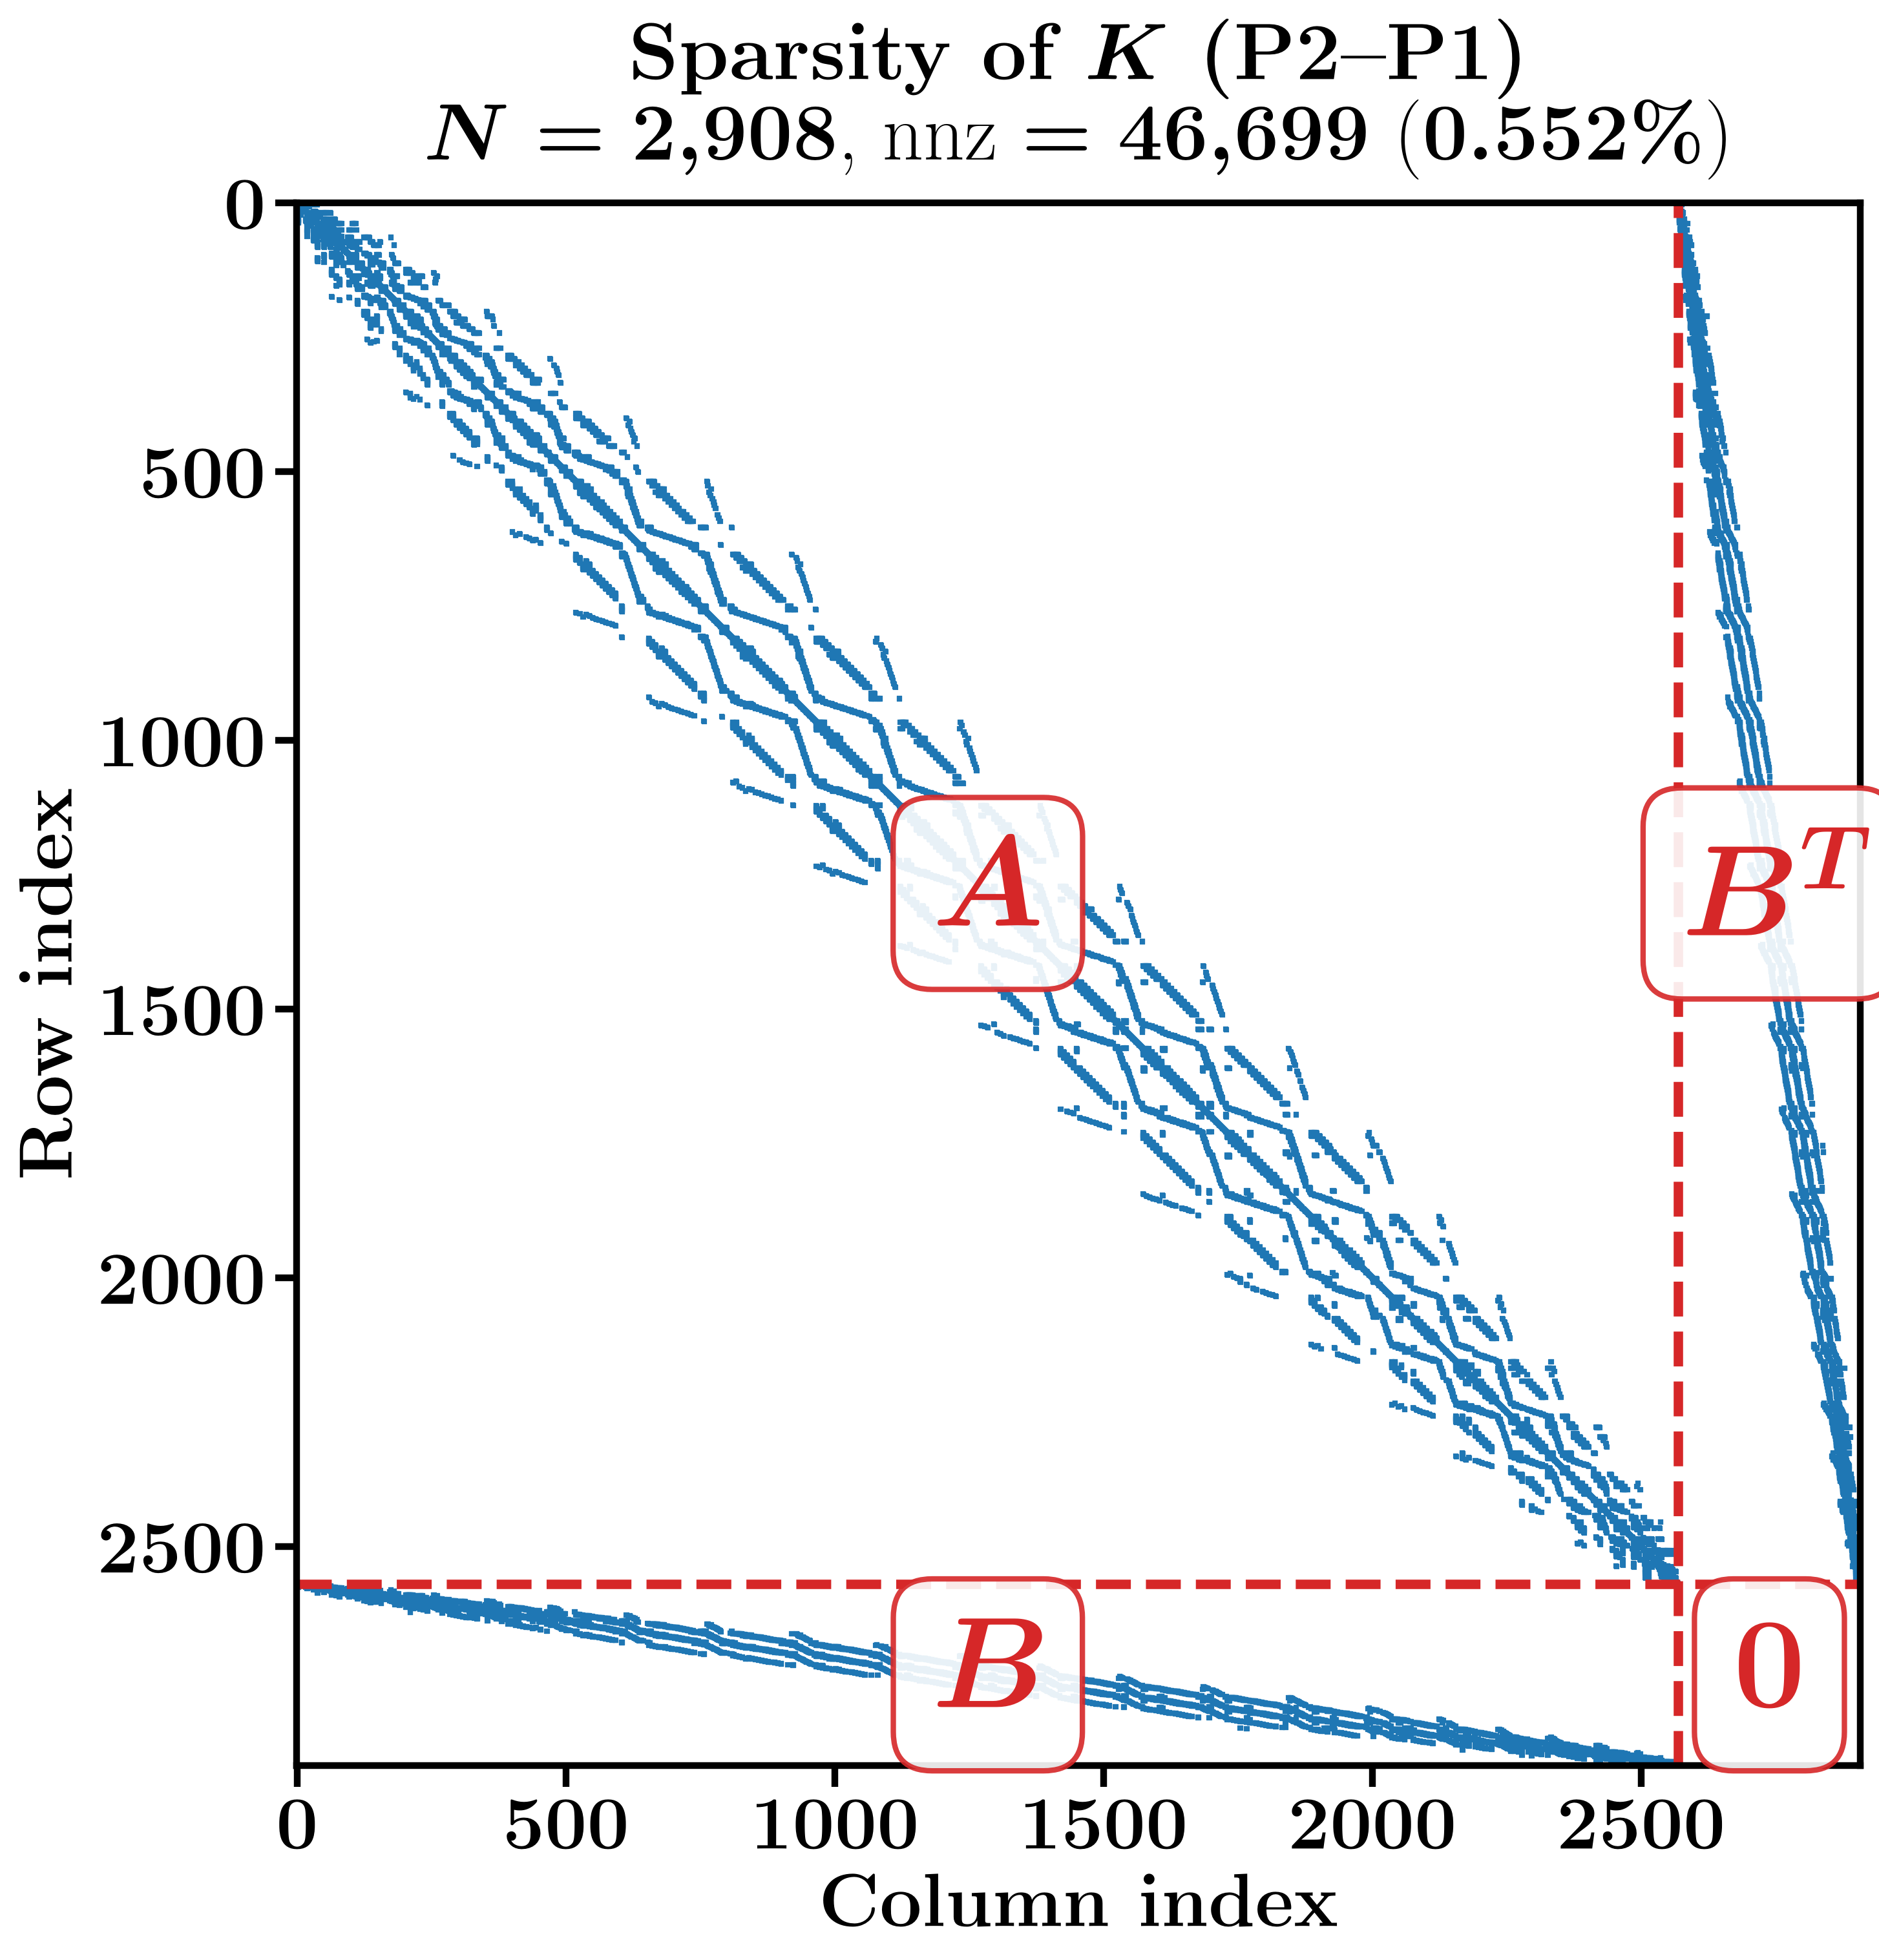
\includegraphics[height=0.9\textheight]{./images/matrix_sparsity.png}
\end{frame}

\begin{frame}{\Large Possible basis elements}
  \Large
  \begin{itemize}
    \item FEM elements library: defelement.org
    \item 67 different elements listed
    \item ones used for investigation: P2-P1, P1-P1, P1b-P1
  \end{itemize}
\end{frame}

\begin{comment}
\begin{frame}{\Large Elements visualized}
  \centering
 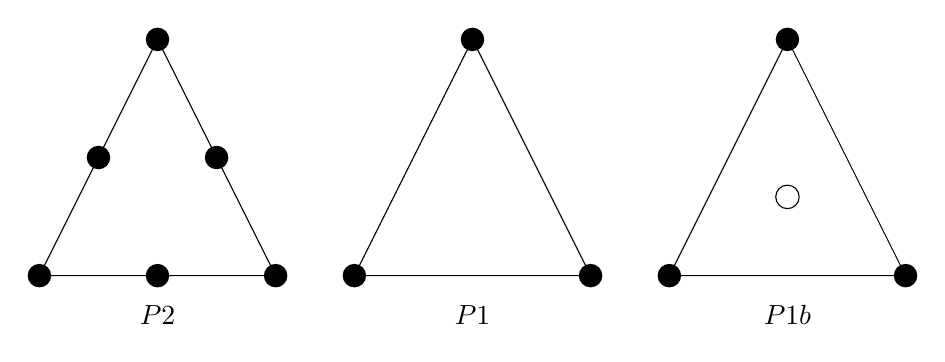
\begin{tikzpicture}[
  dot/.style={circle, fill=black, inner sep=3pt},
  open_circle/.style={circle, draw=black, fill=white, inner sep=3pt},
]

% --- P2: Triangle with six nodes ---
\draw (0,0) -- (3,0) -- (1.5,3) -- cycle;

\node[dot] at (0,0) {};
\node[dot] at (1.5,0) {};
\node[dot] at (0.75,1.5) {};
\node[dot] at (2.25,1.5) {};
\node[dot] at (3,0) {};
\node[dot] at (1.5,3) {};

\node at (1.5,-0.5) {$P2$};

% --- P1: Triangle with three nodes ---
\draw (4,0) -- (7,0) -- (5.5,3) -- cycle;

\node[dot] at (4,0) {};
\node[dot] at (7,0) {};
\node[dot] at (5.5,3) {};

\node at (5.5,-0.5) {$P1$};

% --- P1b: Triangle with three vertices and three edge nodes ---
\draw (8,0) -- (11,0) -- (9.5,3) -- cycle;

\node[dot] at (8,0) {};
\node[dot] at (11,0) {};
\node[dot] at (9.5,3) {};

% Mid-edge nodes
\node[open_circle] at (9.5,1) {};

\node at (9.5,-0.5) {$P1b$};

\end{tikzpicture}
\end{frame}
\end{comment}

\begin{frame}{\Large Stable and unstable solutions}
  \centering
  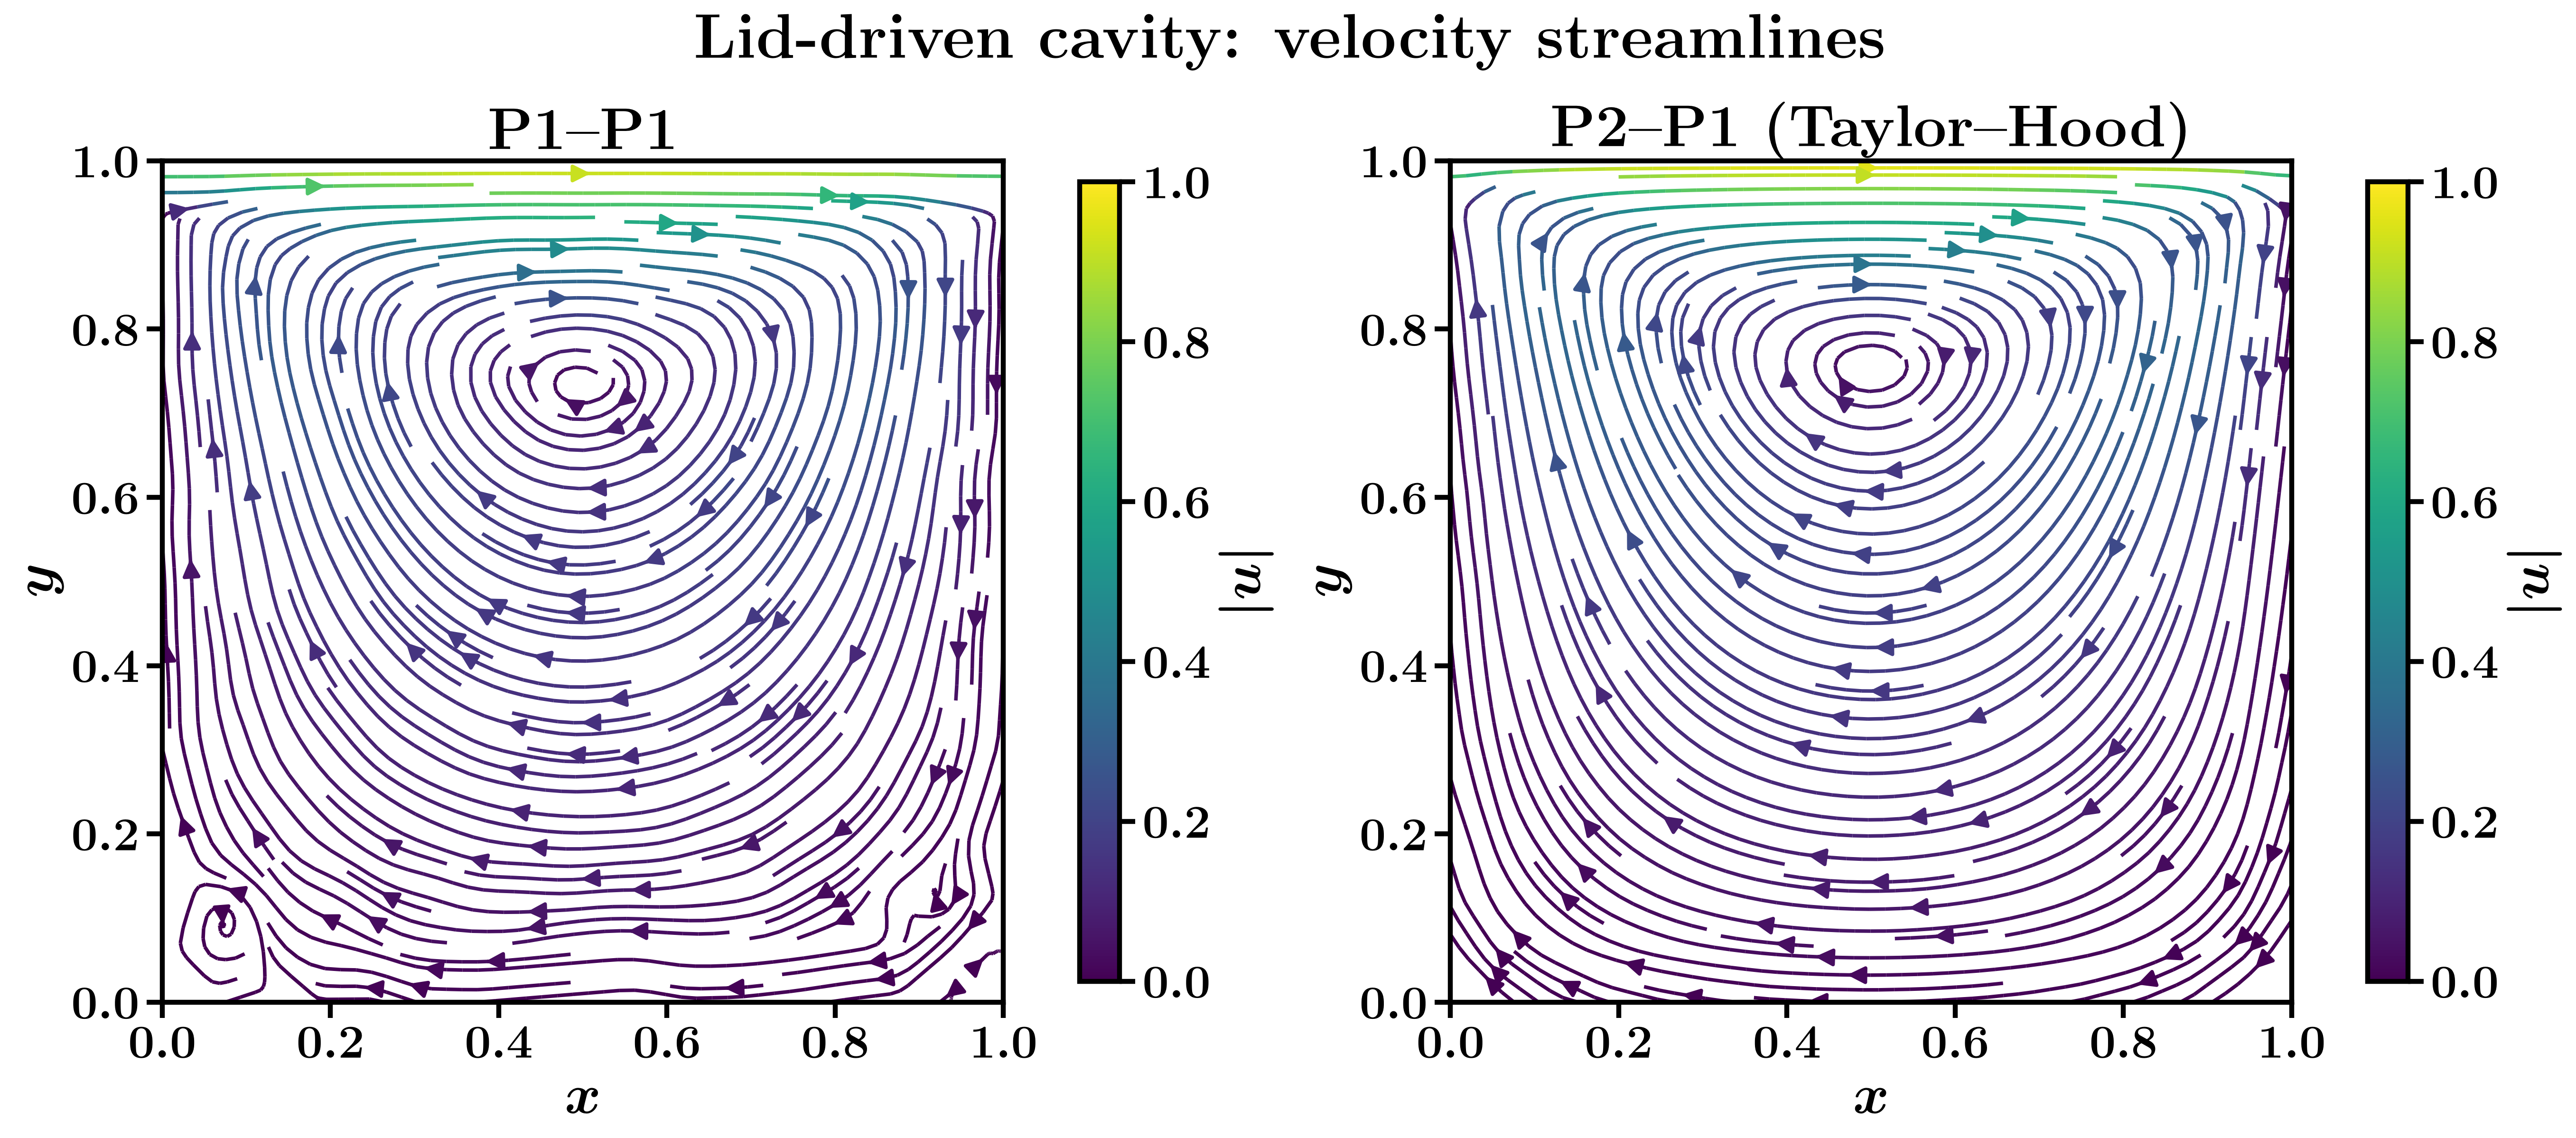
\includegraphics[height=0.85\textheight]{./images/streamlines_comparison.png}
\end{frame}

\begin{frame}{\Large Stable and unstable solutions}
  \centering
  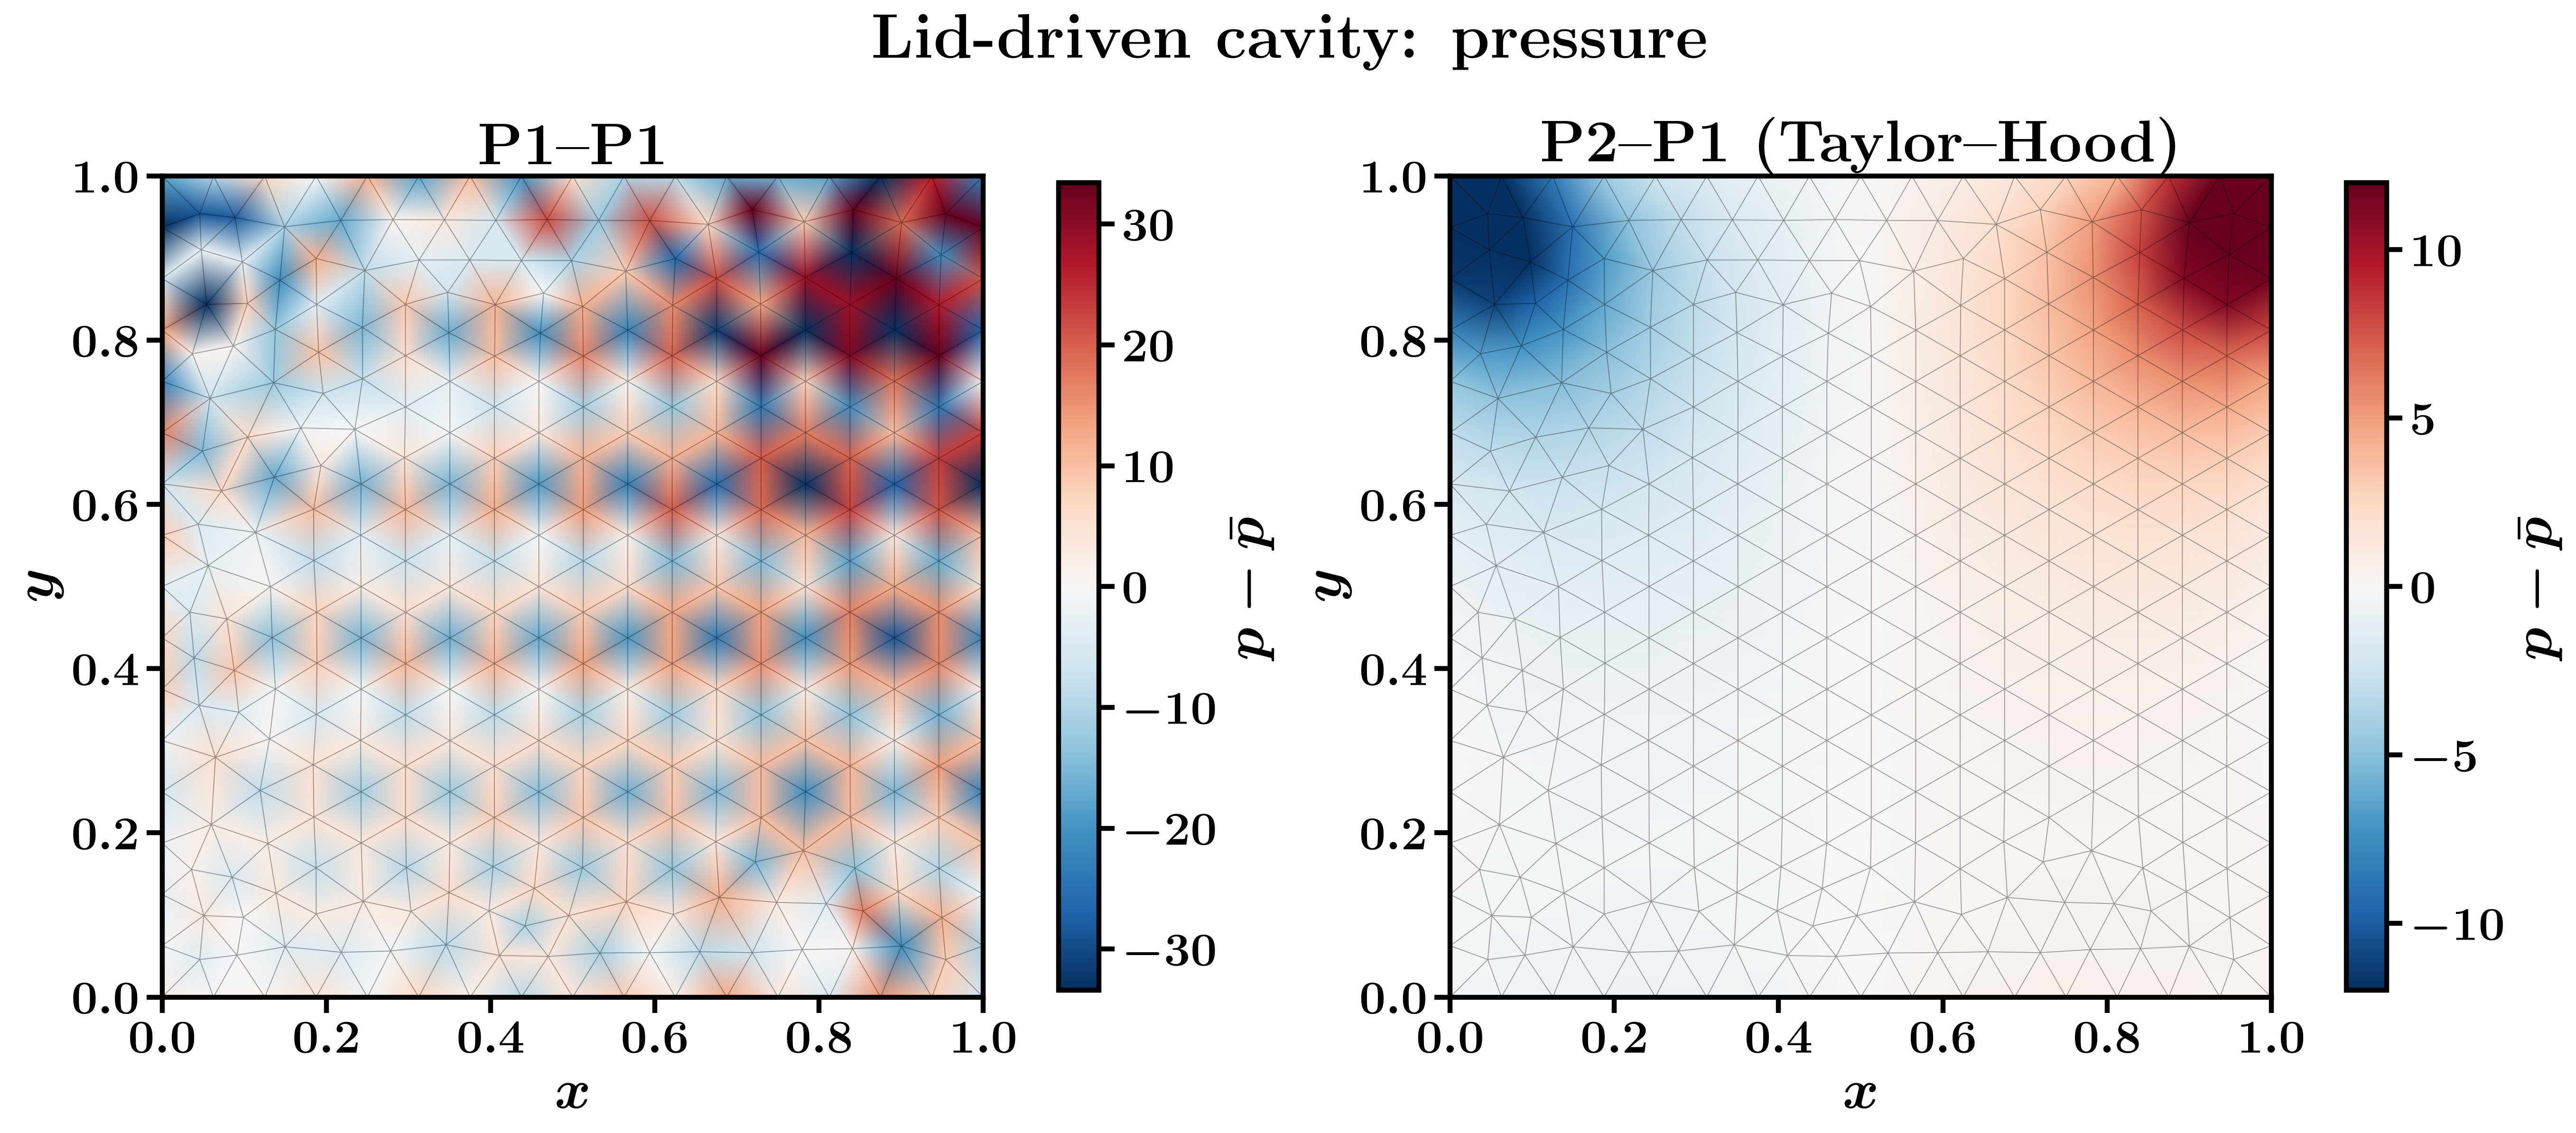
\includegraphics[height=0.85\textheight]{./images/pressure_comparison.png}
\end{frame}

\begin{frame}{\Large Code validation - manufactured solutions}
  \Large
Take a known solution and plug it into existing code
\[
  \mathbf{u}(\mathbf{x}) =
  \pi \begin{pmatrix}
     \sin(\pi x_1)\cos(\pi x_2) \\
    -\cos(\pi x_1)\sin(\pi x_2)
  \end{pmatrix},
  \qquad
  p(\mathbf{x}) = \cos(\pi x_1)\cos(\pi x_2).
\]
\begin{center}
  derived from $\psi(\mathbf{x}) = \sin(\pi x_1)\sin(\pi x_2)$ via
  $\mathbf{u} = (\partial_{x_2}\psi,\, -\partial_{x_1}\psi)^T$,
  so $\operatorname{div}\mathbf{u} = 0$ and $\int_\Omega p = 0$.
\end{center}
\end{frame}

\begin{frame}{\Large A priori error estimates}
  \large
\textbf{1. Quasi-optimality} \hfill {\small (inf-sup stability)}
\[
  |\mathbf{u}-\mathbf{u}_h|_{H^1} + \|p-p_h\|_{L^2}
  \le C(\beta)\Big(\inf_{\mathbf{v}_h\in V_h}|\mathbf{u}-\mathbf{v}_h|_{H^1}
  + \inf_{q_h\in Q_h}\|p-q_h\|_{L^2}\Big)
\]

\textbf{2. Approximation} \hfill {\small (Bramble--Hilbert, shape regularity)}
\[
  |\mathbf{u}-I_h\mathbf{u}|_{H^1} \le C h^{k}|\mathbf{u}|_{H^{k+1}},
  \qquad
  \|p-I_h p\|_{L^2} \le C h^{k}|p|_{H^{k}}
\]

\textbf{3. Duality} \hfill {\small (Aubin--Nitsche, $\Omega$ convex)}
\[
  \|\mathbf{u}-\mathbf{u}_h\|_{L^2}
  \le C h\,\big(|\mathbf{u}-\mathbf{u}_h|_{H^1} + \|p-p_h\|_{L^2}\big)
\]
\end{frame}

\begin{frame}{\Large Expected convergence rates: Taylor--Hood $P_2/P_1$}
  \Large
\[
  |\mathbf{u}-\mathbf{u}_h|_{H^1} + \|p-p_h\|_{L^2} \le C h^{2},
  \qquad
  \|\mathbf{u}-\mathbf{u}_h\|_{L^2} \le C h^{3}
\]

\begin{center}
\begin{tabular}{lcc}
  \hline
  Error & Expected rate & Comes from \\
  \hline
  $|\mathbf{u}-\mathbf{u}_h|_{H^1}$  & $2$ & steps 1 + 2 \\
  $\|p-p_h\|_{L^2}$                  & $2$ & steps 1 + 2 \\
  $\|\mathbf{u}-\mathbf{u}_h\|_{L^2}$ & $3$ & step 3 \\
  \hline
\end{tabular}
\end{center}
\end{frame}

\begin{frame}{\Large Expected convergence rates: Taylor--Hood $P_2/P_1$}
  \centering
  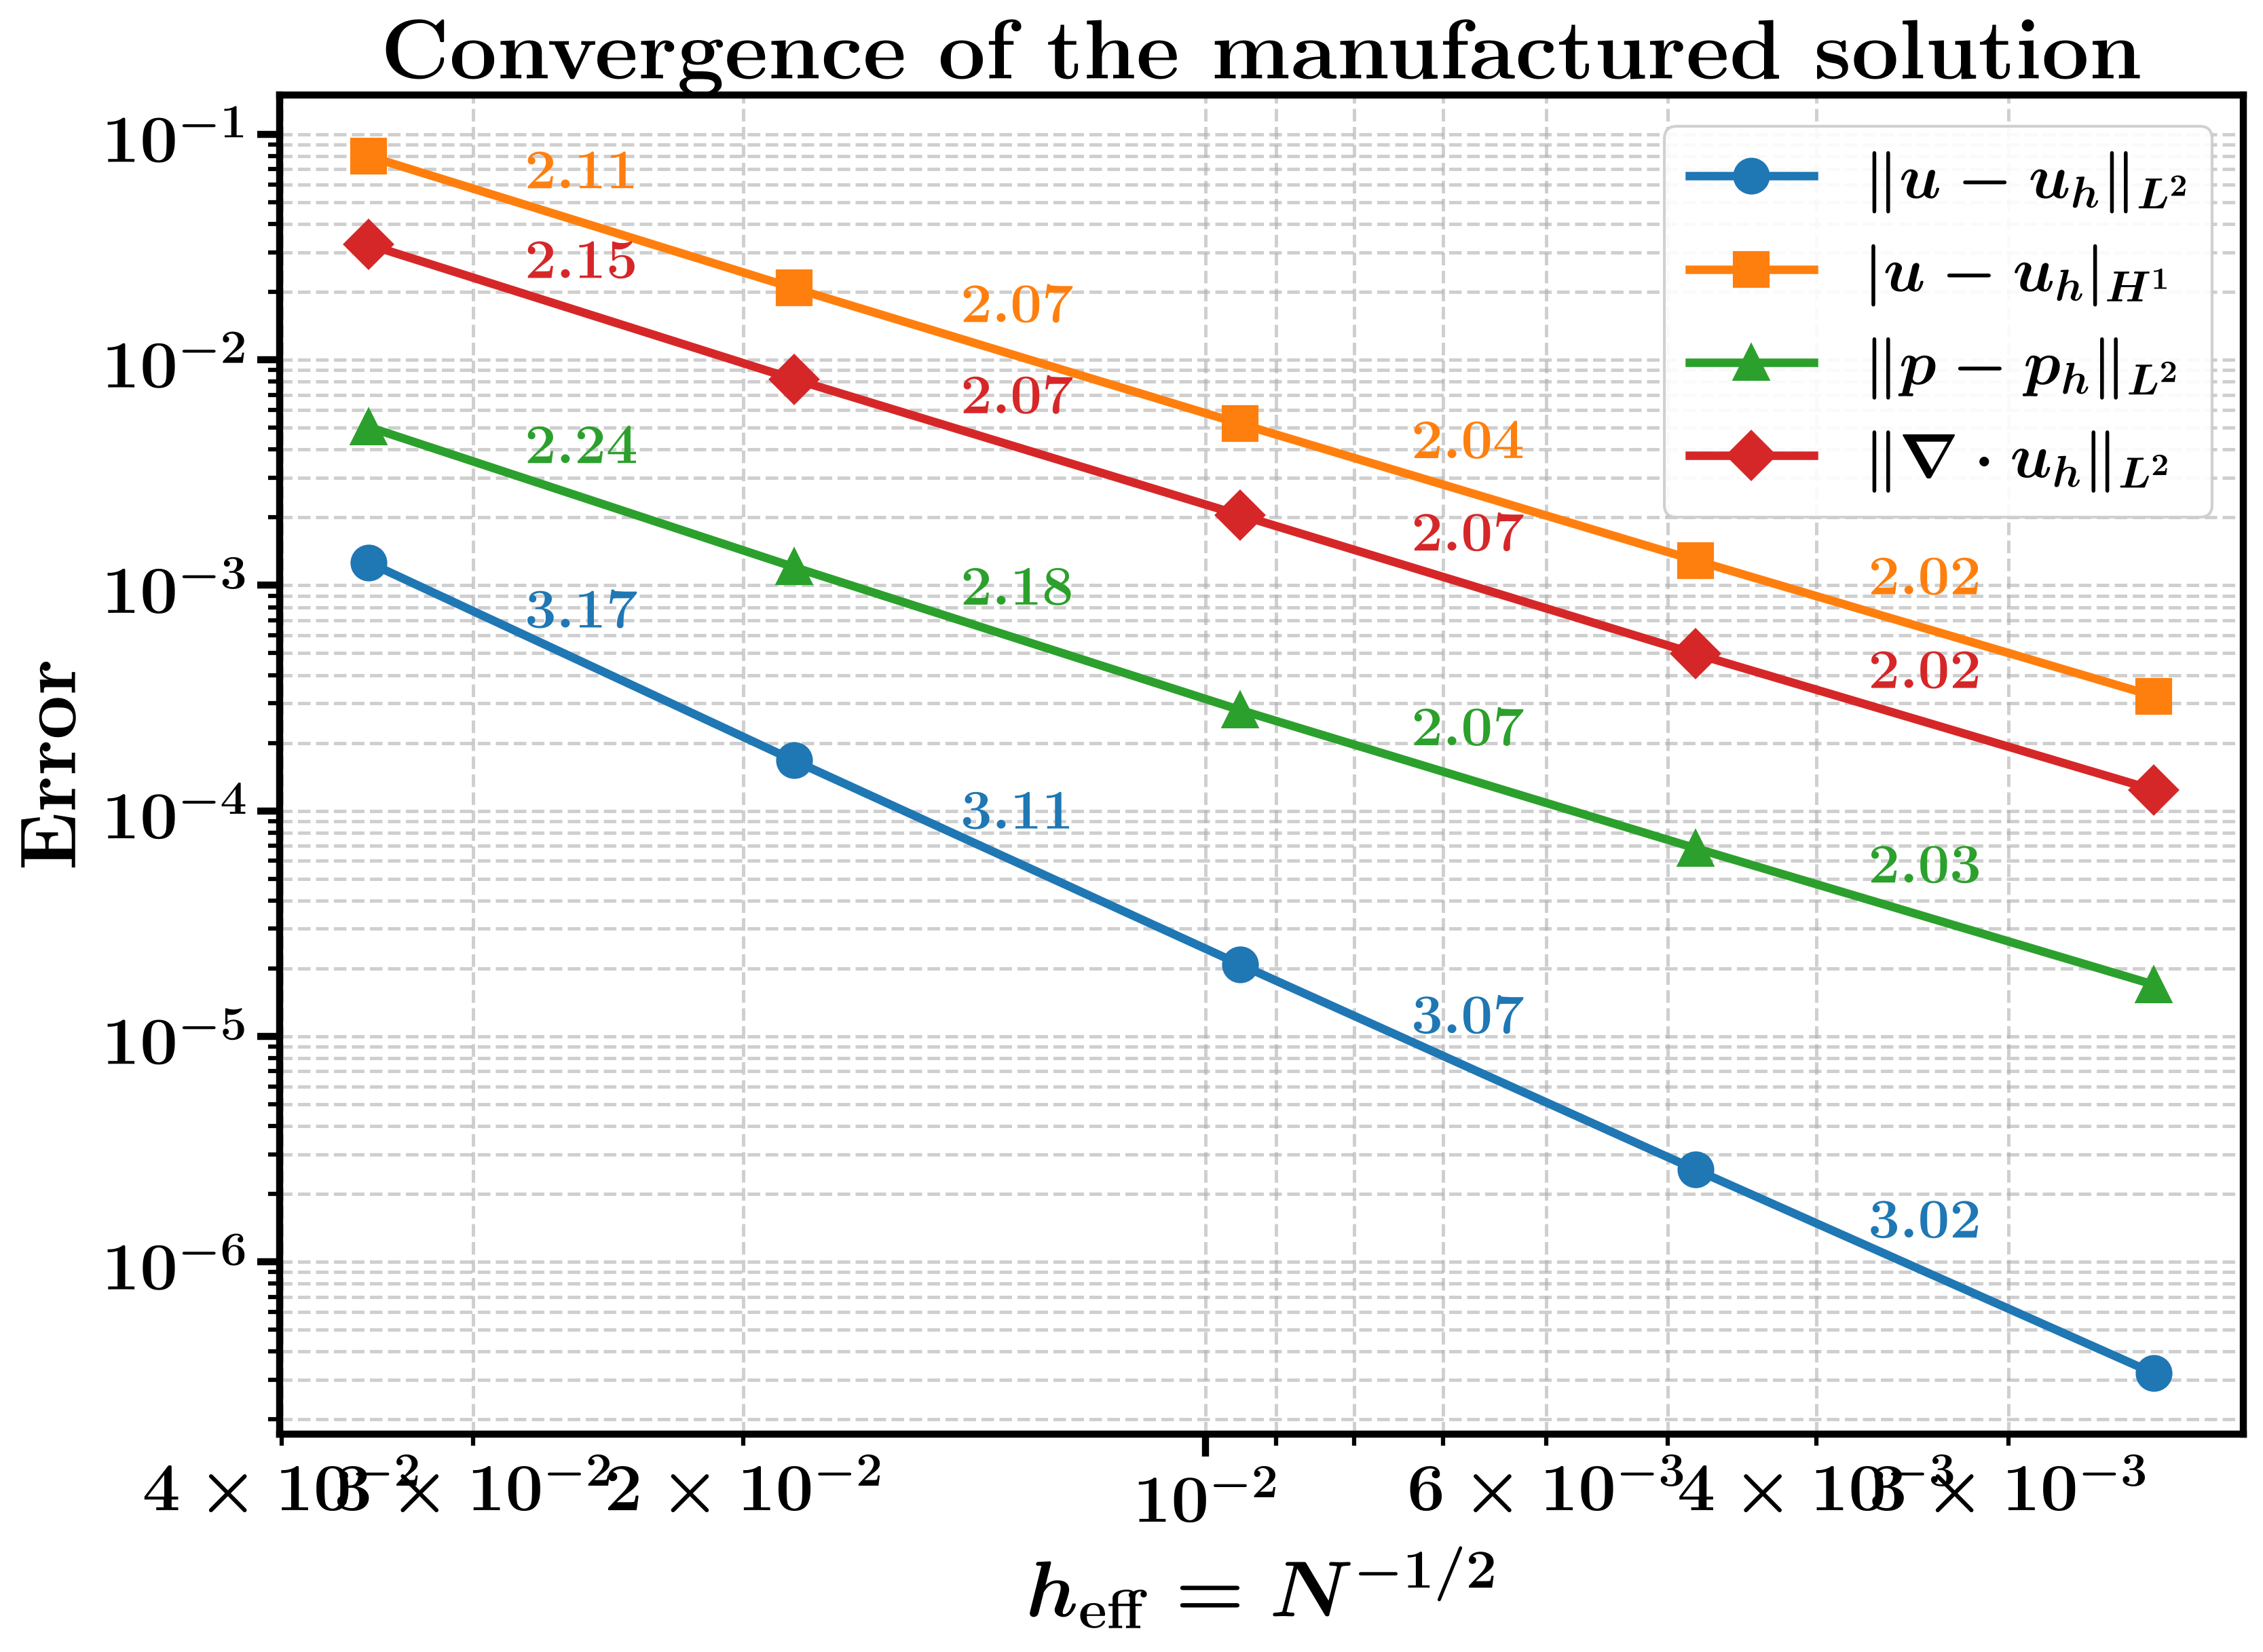
\includegraphics[height=0.9\textheight]{./images/errors.png}
\end{frame}


\begin{comment}
\begin{frame}{\Large Element comparisons}
  \Large
  DOF comparison between the elements for two grid sizes
  \begin{columns}[T]
    \begin{column}{0.48\textwidth}
      $h = 1/32$
      \begin{itemize}
        \item P2-P1: 9834
        \item P1-P1: 2524
        \item P1b-P1: 7312
      \end{itemize}
    \end{column}

    \begin{column}{0.48\textwidth}
      $h = 1/128$
      \begin{itemize}
        \item P2-P1: 152890
        \item P1-P1: 38480
        \item P1b-P1: 114412
      \end{itemize}
    \end{column}
  \end{columns}
\end{frame}
\end{comment}

\begin{frame}{\Large PETSc}
  \Large
  \begin{itemize}
    \item scientific computation toolkit
    \item linear and nonlinear equation solvers
    \item ODE integrators
    \item optimization algorithms
    \item C, Python, Fortran
    \item GPU integration and parallelism
  \end{itemize}
\end{frame}

\begin{frame}{\Large Linear solver algorithms - LU factorisation}
  \Large
  Elimination creates new connections creating fill-in

  \begin{columns}[c]
    
    % Column 1: 5x5 Sparse Matrix
    \begin{column}{0.48\textwidth}
      \centering
      \textbf{Symmetric Matrix $A$}
      \[
      \begin{bmatrix}
        a_{11} & a_{12} & a_{13} & 0 & a_{15} \\
        a_{21} & a_{22} & 0 & a_{24} & 0 \\
        a_{31} & 0 & a_{33} & a_{34} & a_{35} \\
        0 & a_{42} & a_{43} & a_{44} & 0 \\
        a_{51} & 0 & a_{53} & 0 & a_{55}
      \end{bmatrix}
      \]
    \end{column}

    % Column 2: Graph with Chords
    \begin{column}{0.48\textwidth}
      \centering
      \textbf{Undirected Graph $\mathcal{G}(A)$}
      \vspace{0.8em}
      
      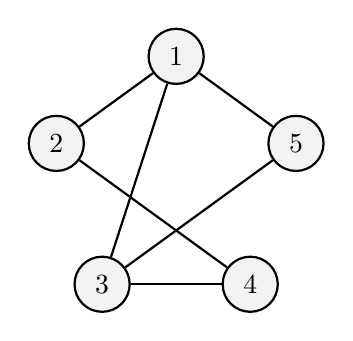
\begin{tikzpicture}[
        main/.style={circle, draw, thick, inner sep=0pt, minimum size=7mm, fill=gray!10},
        edge/.style={thick}
      ]
        % Pentagon Layout
        \node[main] (1) at (90:1.6cm) {$1$};
        \node[main] (2) at (162:1.6cm) {$2$};
        \node[main] (3) at (234:1.6cm) {$3$};
        \node[main] (4) at (306:1.6cm) {$4$};
        \node[main] (5) at (18:1.6cm)  {$5$};

        % Non-cycle / Chordal Edges
        \draw[edge] (1) -- (2); % a_12
        \draw[edge] (1) -- (3); % a_13 (Cross-connection / chord)
        \draw[edge] (1) -- (5); % a_15
        \draw[edge] (2) -- (4); % a_24 (Cross-connection)
        \draw[edge] (3) -- (4); % a_34
        \draw[edge] (3) -- (5); % a_35 (Cross-connection)
      \end{tikzpicture}
    \end{column}

  \end{columns}
\end{frame}

\begin{comment}
\begin{frame}{\Large Linear solver algorithms - LU factorisation}
  \centering
  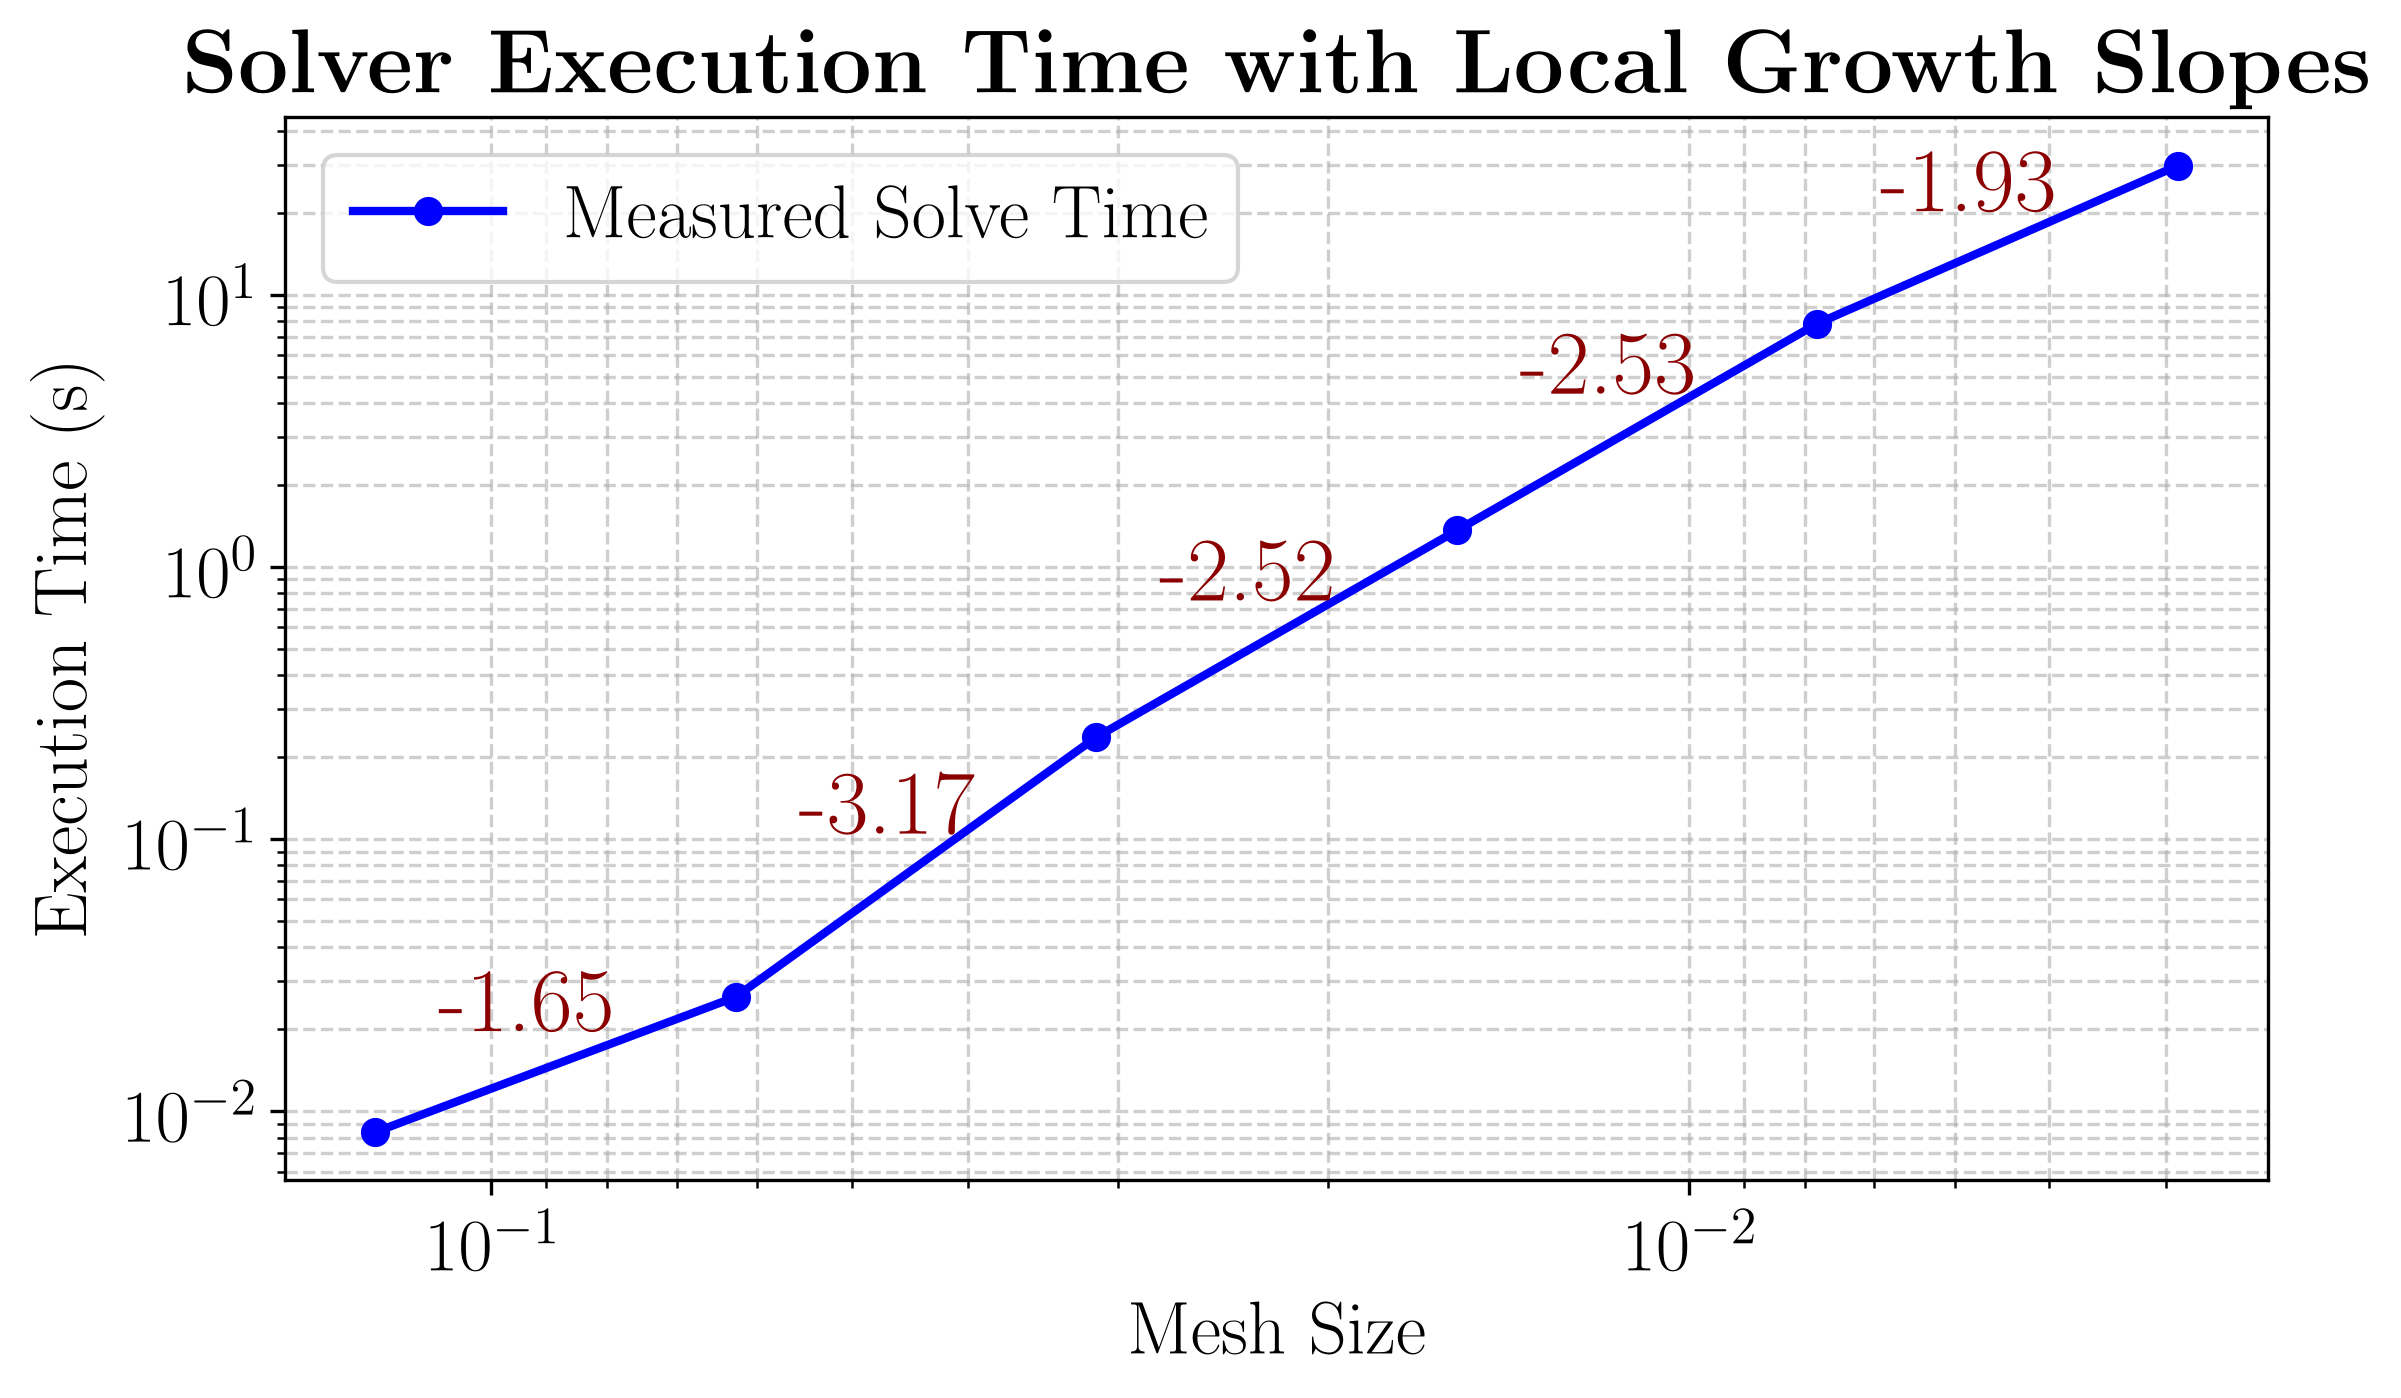
\includegraphics[height=0.85\textheight]{./images/execution_time_LU.png}
\end{frame}
\end{comment}

\begin{frame}{\Large Linear solver algorithms - Krylov methods}
  \Large
  Iteratively solve $A \mathbf{x} = \mathbf{b}$ such that $k$th iterate
  $\mathbf{x}^{(k)}$ lies in the Krylov space:
  \begin{equation*}
    \mathbf{x}^{(0)} + \operatorname{span} \{\mathbf{r}^{(0)}, A\mathbf{r}^{(0)}, A^2\mathbf{r}^{(0)}, \cdots, A^{k-1}\mathbf{r}^{(0)}\}
  \end{equation*}
  where $\mathbf{r}^{(0)} = \mathbf{b} - A \mathbf{x}^{(0)}$.
\end{frame}

\begin{frame}{\Large MINRES}
  \Large
\[
  \mathbf{x}^{(k)} = \operatorname*{arg\,min}_{\mathbf{x}\,\in\,\mathbf{x}^{(0)}+\mathcal{K}_k}
  \|\mathbf{b} - A\mathbf{x}\|_2
\]

\vspace{1em}
\begin{itemize}
  \item symmetric indefinite systems
  \item short recurrence (Lanczos)
  \item preconditioner
    $\mathcal{P} = \begin{pmatrix} \hat A & 0 \\ 0 & \hat M_p \end{pmatrix}$
\end{itemize}
\end{frame}

\begin{frame}{\Large Preconditioning}
  \Large
Solving $A\mathbf{x} = \mathbf{b}$ may be ill-conditioned.
Hence apply $P^{-1}$, thus the system becomes
\[
  P^{-1}A\mathbf{x} = P^{-1}\mathbf{b}.
\]

Choose $P$ such that
\begin{itemize}
  \item eigenvalues of $P^{-1}A$ are clustered
  \item $P^{-1}\mathbf{v}$ is cheap to compute
  \item $P$ is SPD \hfill {\small (required by MINRES)}
\end{itemize}
\end{frame}

\begin{frame}{\Large Field-split preconditioning}
  \Large
\[
  \mathcal{A} = \begin{pmatrix} A & B^{T} \\ B & 0 \end{pmatrix},
  \qquad
  \mathcal{P} = \begin{pmatrix} \hat A & 0 \\ 0 & \hat M_p \end{pmatrix}
\]

\vspace{1em}
\begin{center}
\begin{tabular}{ll}
  \texttt{additive} & block diagonal \\[0.3em]
  $\hat A$          & one AMG V-cycle (\texttt{gamg}) \\[0.3em]
  $\hat M_p$        & $\operatorname{diag}(M_p)$ (\texttt{jacobi})
\end{tabular}
\end{center}
\end{frame}

\begin{frame}{\Large Expected computational cost}
  \Large
\begin{center}
\begin{tabular}{lcc}
  \hline
  Solver & Time & Memory \\
  \hline
  LU (MUMPS)              & $O(n^{3/2})$ & $O(n\log n)$ \\[0.3em]
  MINRES + field-split    & $O(n)$       & $O(n)$ \\
  \hline
\end{tabular}
\end{center}

\vspace{1em}
\[
  \text{slope in } \log T \text{ vs.\ } \log n: \qquad
  \text{LU} \approx 1.5, \qquad \text{MINRES} \approx 1
\]
\end{frame}

\begin{frame}{\Large Solver algorithms compared}
  \centering
  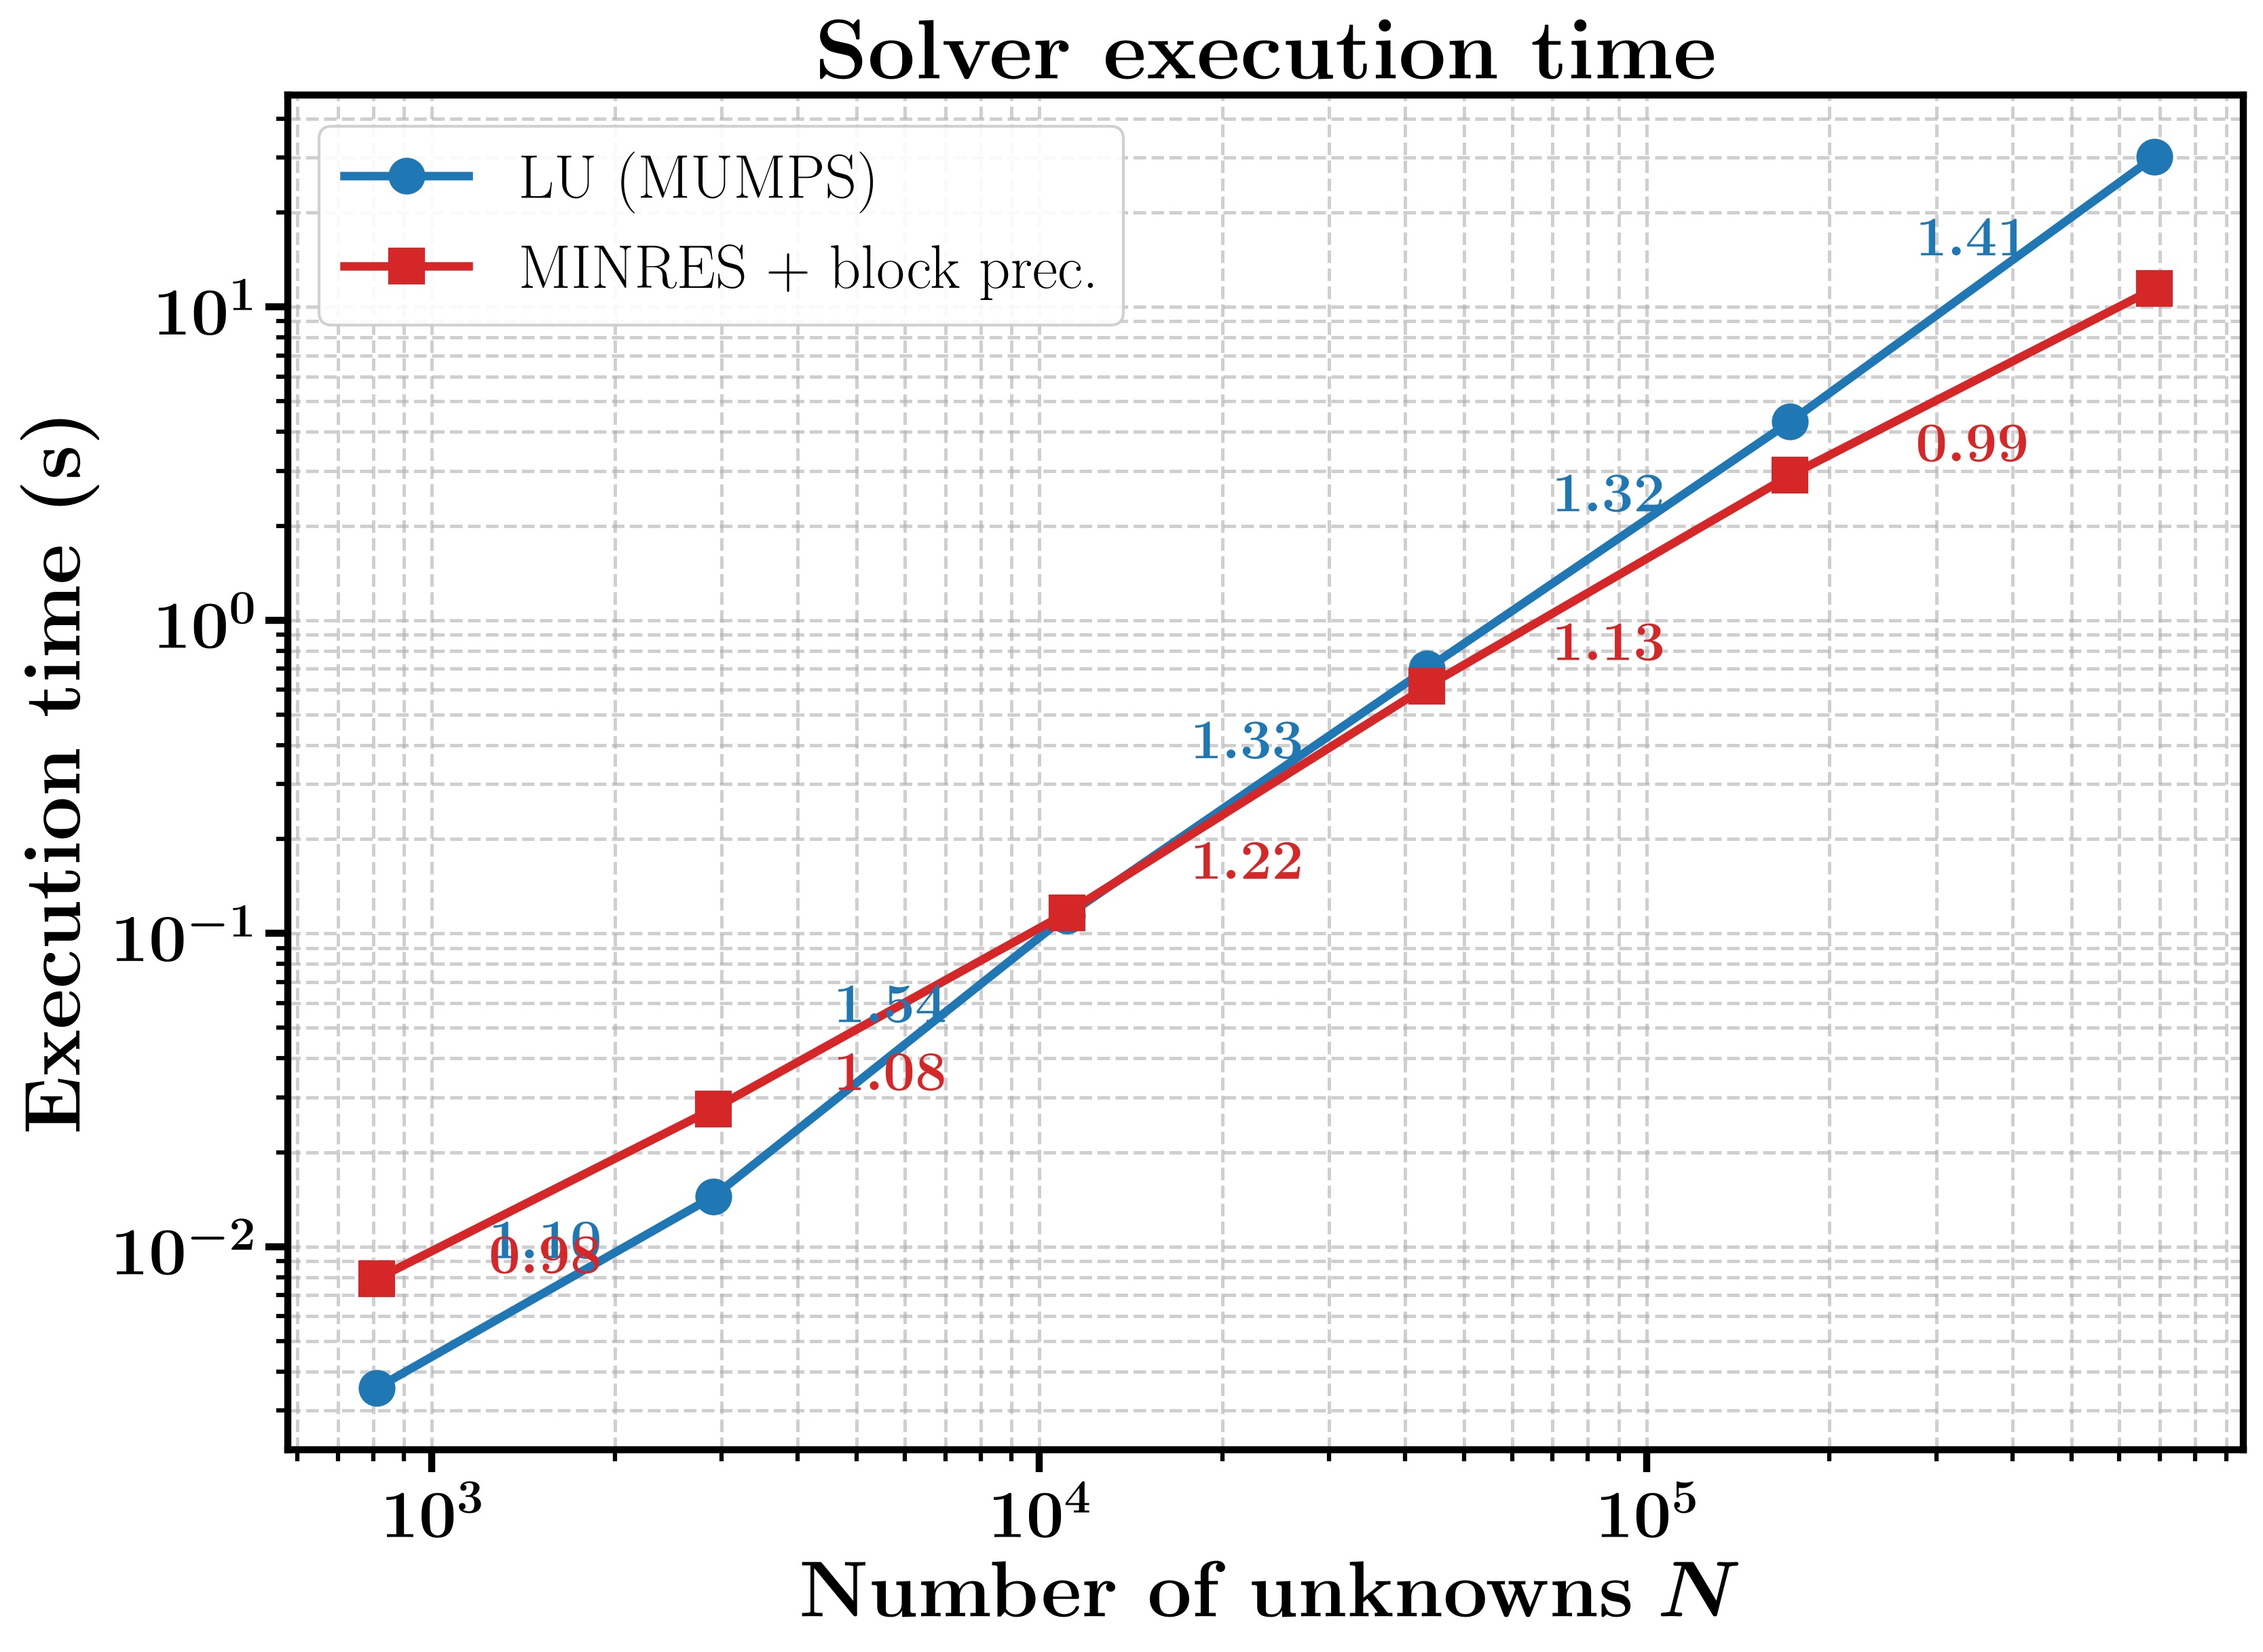
\includegraphics[height=0.9\textheight]{./images/execution_time.png}
\end{frame}

\begin{frame}{\Large Solver algorithms compared}
  \centering
  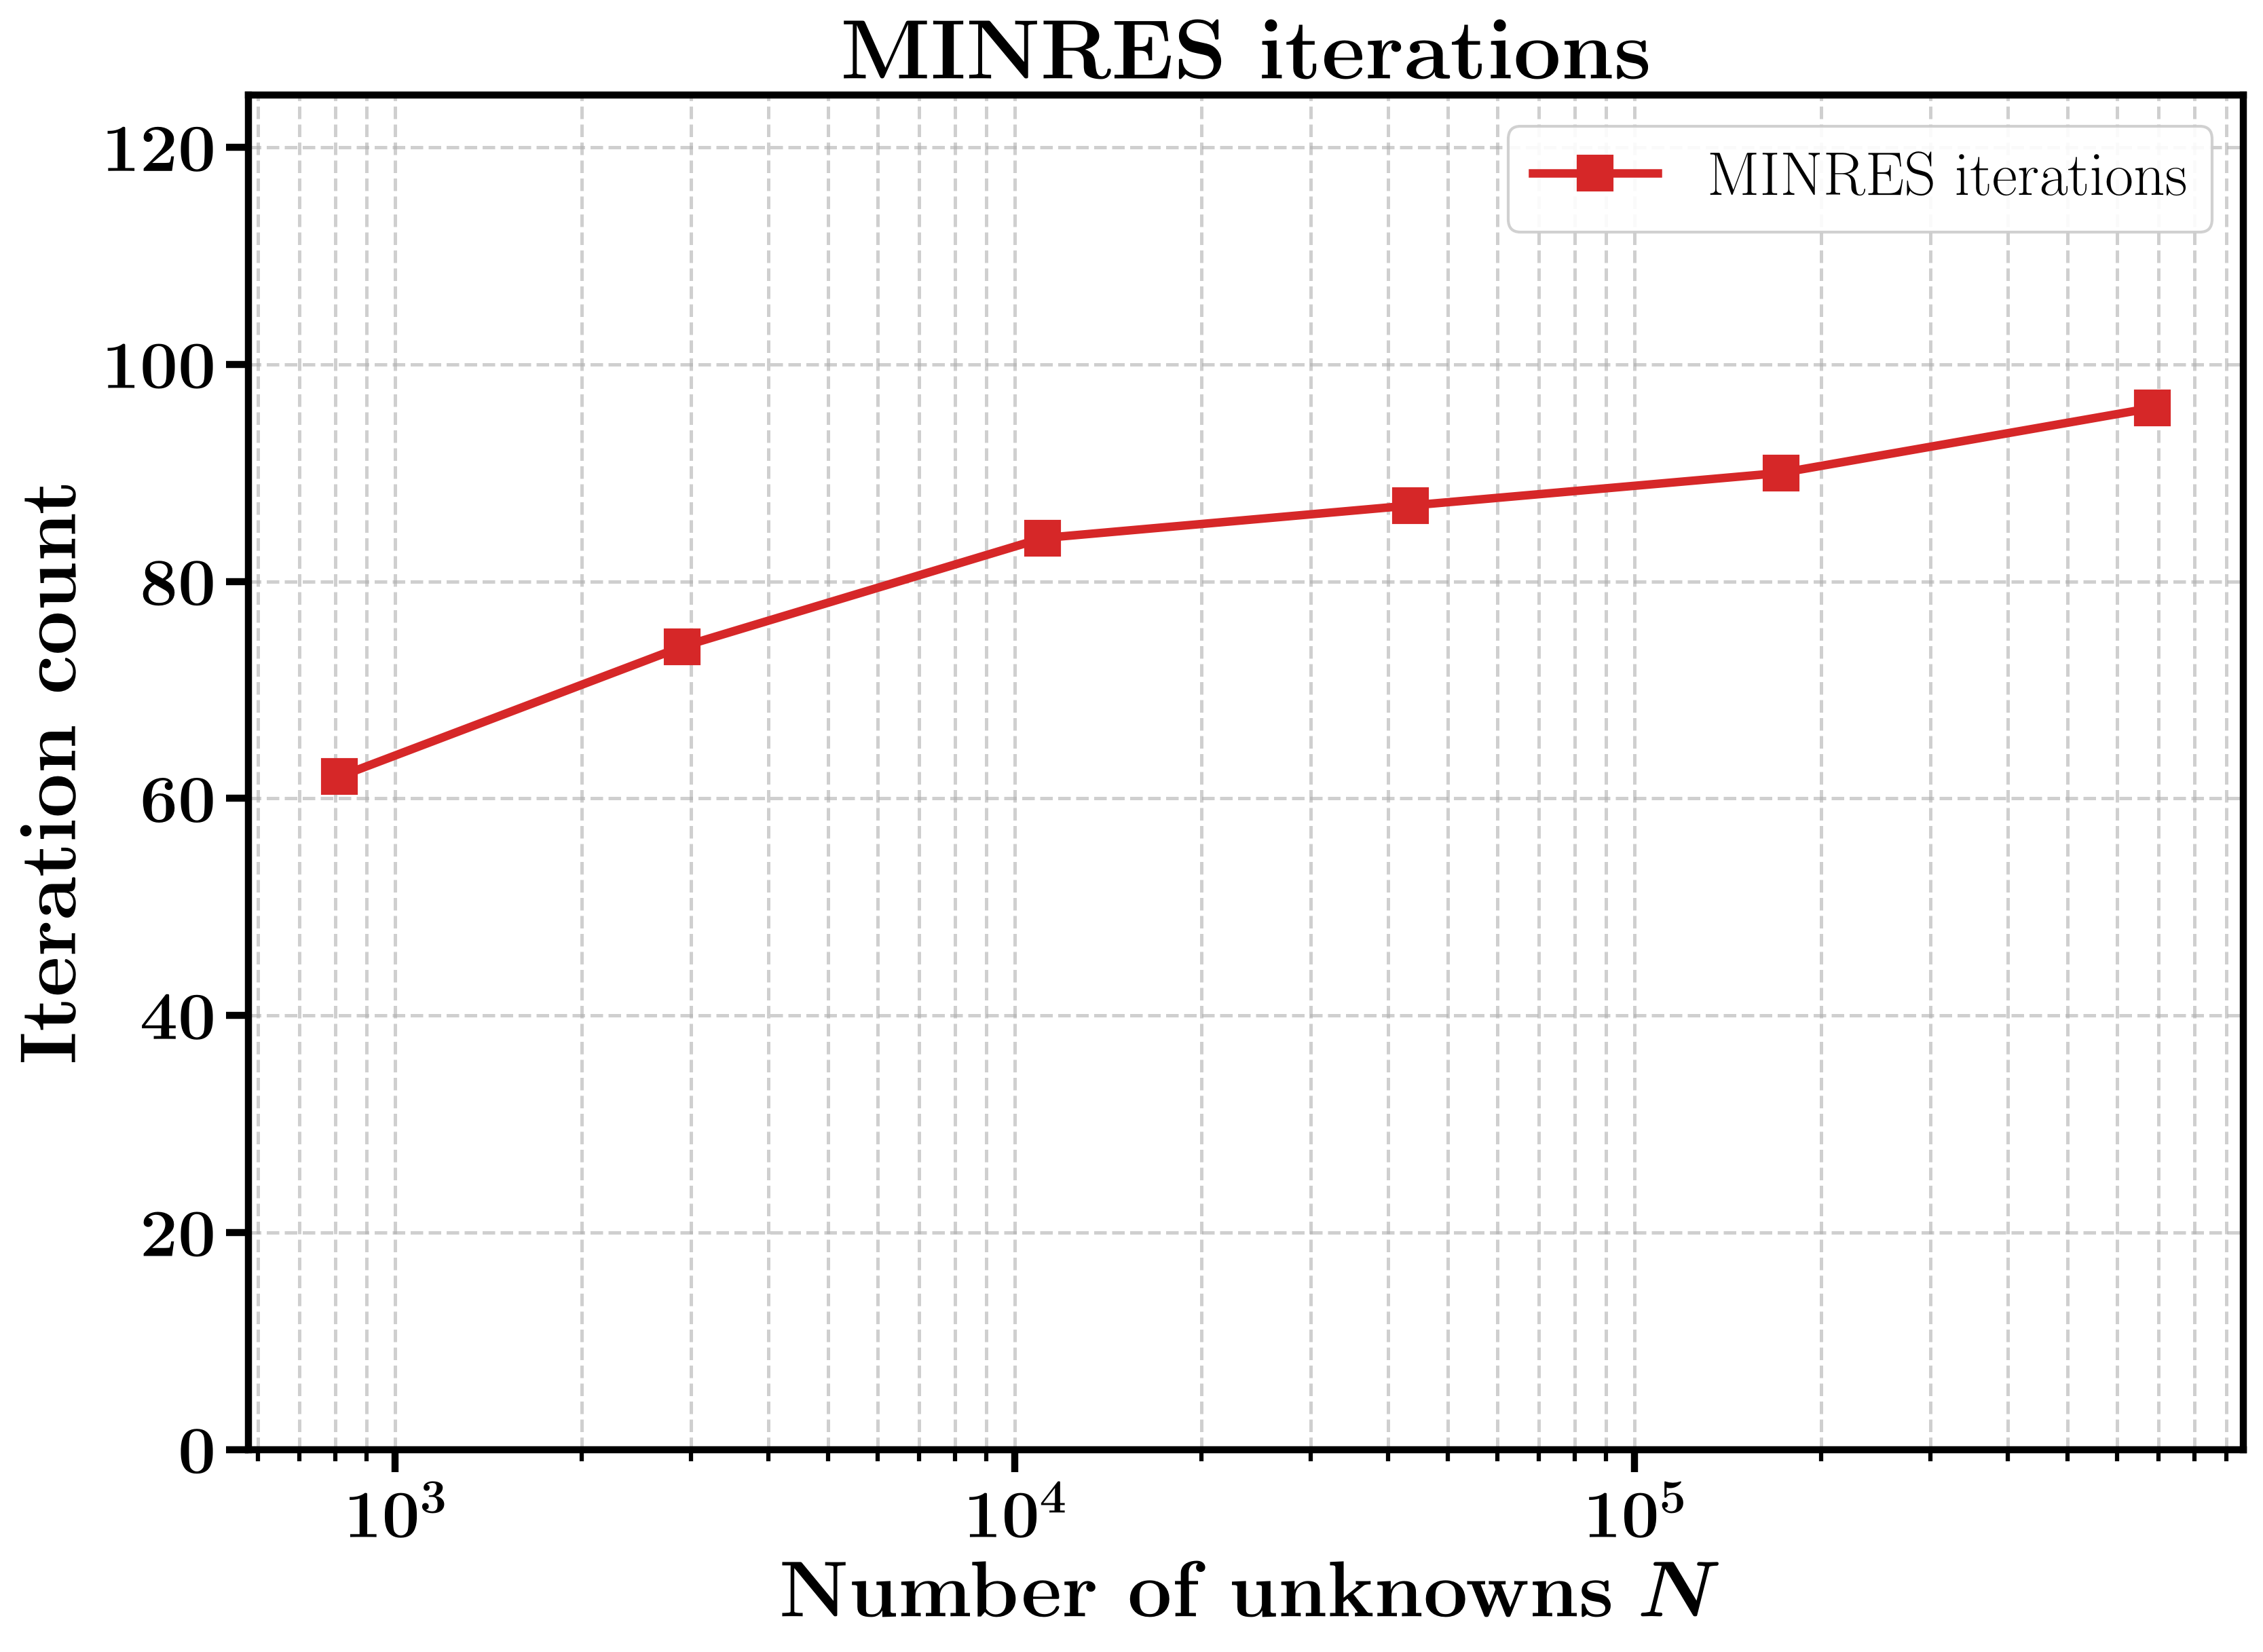
\includegraphics[height=0.9\textheight]{./images/iterations_MINRES.png}
\end{frame}

\begin{comment}
\begin{frame}{\Large Manufactured solutions failure}
  \centering
  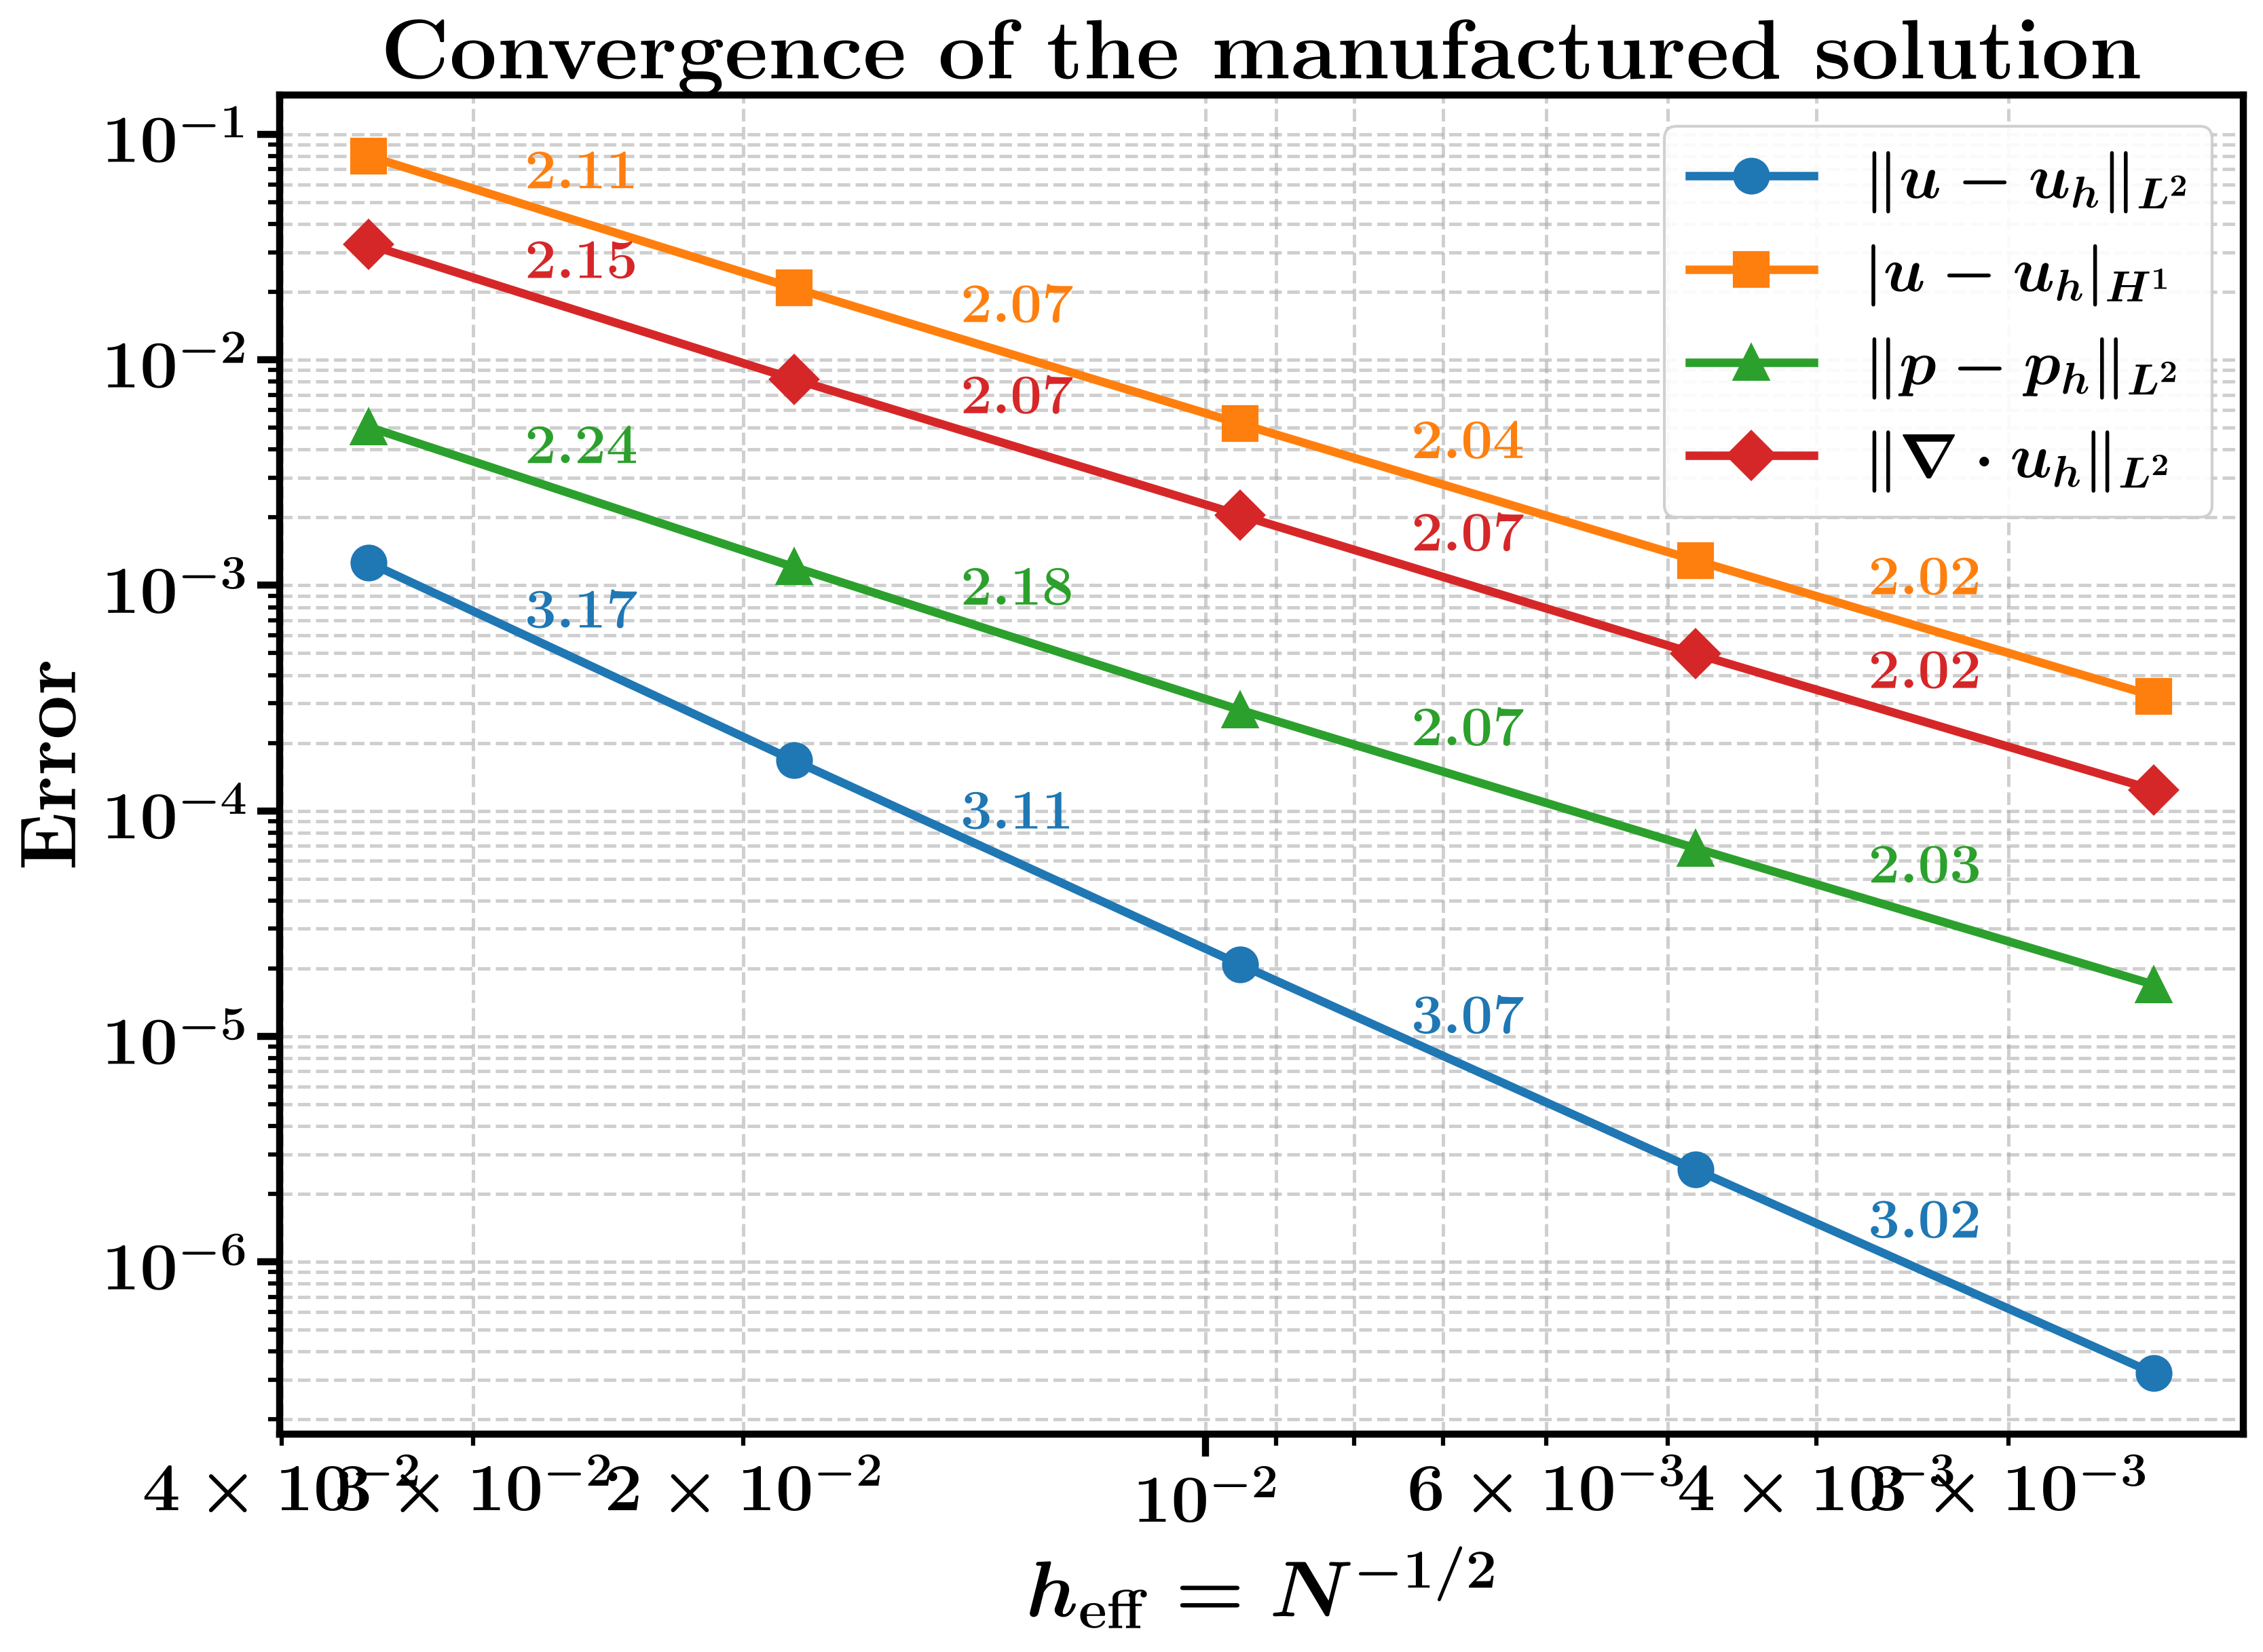
\includegraphics[height=0.85\textheight]{./images/errors.png}
\end{frame}
\end{comment}

\begin{frame}{\Large Reflections on AI use}
  \Large
  \begin{enumerate}
    \item General topic research: valuable
    \item Brainstorming, reasoning check: great
    \item Coding simple scripts: efficient
    \item Coding niche requirements: unsatisfactory
  \end{enumerate}
\end{frame}

\begin{frame}[standout]
  Thank you for your attention!
\end{frame}
\end{document}
